%%%%%%%%%%%%%%%%%%%%%%%%%%%%%%%%%%%%%%%%%%%%%%%%%%%%%%%%%%%%%%%%%%%%%%%%%
%                                                                       %
%              A template file for usage with ustthesis.cls             %
%                                                                       %
%%%%%%%%%%%%%%%%%%%%%%%%%%%%%%%%%%%%%%%%%%%%%%%%%%%%%%%%%%%%%%%%%%%%%%%%%

\documentclass[12pt]{ustthesis}

\usepackage{amsmath, amssymb}
\usepackage{algorithm}
\usepackage{algorithmic}
\usepackage{color,graphicx}
\usepackage{siunitx}
\usepackage{soul}
\usepackage{graphics} % for pdf, bitmapped graphics files
\usepackage{subcaption}
\newtheorem{proof}{Proof}
\usepackage{bookmark}
\usepackage{hyperref} % for better viewing experience  -- added by alan
\usepackage{textcomp}
\usepackage{multirow}
\usepackage{nth}
\usepackage{indentfirst}
\usepackage{siunitx}
\usepackage{changepage}
\usepackage[a4paper, margin=1in]{geometry} % page requriement from the university ---added by Lei.
\usepackage{setspace}
% Alan: begin the font trial
% Euler for math | Palatino for rm | Helvetica for ss | Courier for tt
% \renewcommand{\rmdefault}{ppl} % rm

% NOTE Lei: rouphly 32 lines for 12pt font size and 1.5 line spacing
% \linespread{0.5}
\singlespacing
% \onehalfspacing
%\doublespacing

% \usepackage[scaled]{helvet} % ss
% \usepackage{courier} % tt
% \usepackage{euler} % math
% \usepackage{eulervm} % a better implementation of the euler package (not in gwTeX)
% \normalfont
% \usepackage[T1]{fontenc}
% Alan: end the font trial


\DeclareMathOperator*{\argmax}{\arg\!\max}
\DeclareMathOperator*{\argmin}{\arg\!\min}

\newcommand{\red}[1]{#1}
\newcommand{\tab}[1]{\hspace{3mm}}

% NOTE Lei: personal habit for math symbols.
\newcommand{\bx}{\mathbf{x}}
\newcommand{\bX}{\mathbf{X}}
\newcommand{\by}{\mathbf{y}}
\newcommand{\bY}{\mathbf{Y}}
\newcommand{\bD}{\mathbf{D}}
\newcommand{\bE}{\mathbf{E}}
\newcommand{\ba}{\mathbf{a}}
\newcommand{\bs}{\mathbf{s}}
\newcommand{\bn}{\mathbf{n}}
\newcommand{\bI}{\mathbf{I}}
\newcommand{\bsigma}{\mathbf{\sigma}}
\newcommand{\cS}{\mathcal{S}}
\newcommand{\cX}{\mathcal{X}}
\newcommand{\cA}{\mathcal{A}}
\newcommand{\cB}{\mathcal{B}}
\newcommand{\cD}{\mathcal{D}}
\newcommand{\bu}{\mathbf{u}}
\newcommand{\bv}{\mathbf{v}}
\newcommand{\ts}{\textsuperscript}
\newcommand{\etal}{{\em et al.}}
\newcommand{\norm}[1]{\left\lVert#1\right\rVert}
\DeclareMathOperator{\atantwo}{atan2}
\newcommand{\argminE}{\mathop{\mathrm{argmin}}}

\setcounter{tocdepth}{3}
\setcounter{secnumdepth}{3}

% \renewcommand{\familydefault}{\rmdefault}

% \usepackage{latexsym}
    % Use the "latexsym" package when encountering the following error:
    %   ! LaTeX Error: Command \??? not provided in base LaTeX2e.
% \usepackage{epsf}
    % Use the "epsf" package for including EPS files.

%%%%%%%%%%%%%%%%%%%%%%%%%%%%%%%%%%%%%%%%%%%%%%%%%%%%%%%%%%%%%%%%%%%%%%%%%
%                                                                       %
% Preambles. DO NOT ERASE THEM. Change to suite your particular purpose.%
%                                                                       %
%%%%%%%%%%%%%%%%%%%%%%%%%%%%%%%%%%%%%%%%%%%%%%%%%%%%%%%%%%%%%%%%%%%%%%%%%

\title{Vision-Based Localization and Map Update for Long-Term Navigation in Changing Environments}  % Title of the thesis.
\author{Jingwen~YU}     % Author of the thesis.

% NOTE Lei: choose your degree
% \degree{\MPhil}             % Degree for which the thesis is.
% %% or
% \degree{\PhD}              % Degree for which the thesis is.

\department{Electronic and Computer Engineering}       % Department to which the thesis

\advisor{~Prof.~Ming~LIU}     % Supervisor.

% NOTE Lei: Uncomment this line if you have a co-supervisor/co-advisor
\coadvisor{~Prof.~Hong~Zhang}     % Co Supervisor.

% \depthead{Prof.~Meimei~Han}    % department head.

%\defencedate{2019}{08}{05}      % \defencedate{year}{month}{day}   NOTE Lei: change it to the submission month when you submit your final version.

% NOTE:
%   According to the sample shown in the guidelines, page number is
%   placed below the bottom margin.  However, if the author prefers
%   the page number to be printed above the bottom margin, please
%   activate the following command.
% \PNumberAboveBottomMargin

\graphicspath{{./figure/}}
\begin{document}

% abstract of the report
\begin{abstract}
For autonomous robot navigation, vision-based system can be easily deployed with 
inexpensive commercial cameras, especially for monocular visual navigation system. 
However, visual sensors are sensitive to environmental changes caused by lighting, object movement, weathers and seasons.
For both indoor and outdoor autnomous navigation, the changes over time can lead to poor localization
and deterioration in map quality. This may lead to a significant drop on robustness, especially for tasks involving repeated traversals such as autnomous path following, i.e. visual teach and repeat task.
To enable long-term autonomous navigation system, the robustness of the system is a must.
While extensive techniques are proposed to strengthen the robustness of localization
through image retrieval or deep-trained image features that are invariant to appearance changes and viewing angle.
They demonstrate impressive performance on changes caused by lighting condition variantion and seasonal changes, 
while they rarely focus on the changes caused by object movement. This kind of changes are rather typical
in situations such as parking lots, warehouses and offices. The movement can cause not only the appearance change,
but also the infeasibility of the previous paths. In extreme condition, object movement may lead to the
number of features to be insufficient, thus the localization fails.
Besides, localization and mapping are tightly-coupled, however, current researchs lack of an emphasis 
on map managment and update for long-term navigation tasks.
Therefore, this proposal focus on the long-term navigation system enabled by visual sensors and targets on
test and improve the localization robustness under environmental changes aroused by object movements.
Moreover, the corresponding map maintance algorithms aiming at record and update the surrounding changes is 
proposed as an important research direction. With the robustness improvement on localization and
mapping under changing environments, the long-term autnomous navigation tasks e.g. autonomous route following,
should be achieved.
\end{abstract}

% chapter 1, introduction with background, related work 
\chapter{Introduction}
\section{Background}
Autonomous mobile robotic systems are emerging dramatically in recent years from
unmanned aerial vehicles (UAVs) to unmanned ground vehicles (UGVs), from self-driving
vehicle to indoor service robots. A large portion of industrial applications has
already achieved high-level autonomy through state-of-the-art techniques. 
For industrial robots, the operation environment is usually structurally constrained and fixed with various customized assisting modules such as using a pre-installed external visual marker system to assist localization and detection. 
Therefore, the industrial environment is barely changed with high stability, 
while for other demanding scopes of applications (e.g. autonomous driving, warehouse robots, and service robots), the operational surrounding changes significantly with high dynamics and uncertainties. This highlights the key focus on robustness and reliability under changing environments for the wide spread of autonomous mobile robots. In the development of Hercules\cite{liuhercules}, an autonomous vehicle targeting low-speed delivery, the stability under the dynamic environment is demonstrated and emphasized to enable safe autonomy. A picture of Hercules is shown in Fig\ref{fig:Hercules}.

Compared to a 3D laser scanner, also known as Light detection and ranging (LiDAR), 
visual sensors (i.e. cameras) are cheaper and able to provide rich
texture information, which is more suitable for high-level interactive tasks such
as mobile manipulation, and human-robot interaction. Cameras are also lightweight which enables massive and efficient deployment on all kinds of robotic platforms, e.g. on micro aerial robotics. While LiDARs are not suitable for their weight and size, as well as high drive power source requirements. Therefore, vision-based localization and mapping techniques are important which can achieve comparable performance with much lower hardware requirements.

This proposal focuses on the vision-based long-term navigation tasks, which require 
high robustness. During the task completion, the robot might encounter an environment with uncertainty, such as highly dynamic objects (humans, vehicles, and other operating robots), moderately dynamic objects (boxes, bins, and chairs), and static objects but could be changed or moved (fences, wall, and trees). This uncertainty of surrounding changes 
can lead to the failure of localization and inaccuracy of the map. Without a doubt, the localization of robots is the fundamental problem that other operations rely on.
Regarding map accuracy, the incremental changes and possible loss of localization make it important to maintain an up-to-date map. Moreover, the discovery of the human memory system shows the mechanism behind an incrementally and continuous learning system. The human memory system contains temporal memory as well as long-term memory. In 2022, BioSLAM\cite{yin2022bioslam} proposed a dual-memory system for place recognition system to maintain accuracy with various incremental new appearances. Current research seldom tackles this problem while mostly focusing on temporal navigation and assuming the environment to be static. Constrained by real-time computing resources as well as robustness, there is still a large gap toward long-term stable mobile navigation. Inspired by \cite{yin2022bioslam} and \cite{paton2016bridging}, both adopted the idea of building more than one map over the same changing environment, I proposed to carry out further research on strengthening the robustness of long-term perception system by leveraging multiple experiences and traversals over the same place. Specifically, from two perspectives, localization algorithm and map management mechanism.


\section{Related Work}
\subsection{Visual Teach-and-Repeat}
The teach-and-repeat navigation\cite{paul2010vtr,mcmanus2012visual} is one of the basic tasks in mobile robots, which enables a large number of applications such as autonomous delivery, transportation, inspection, and patrolling. As the name suggests, the system contains two phases. In the teaching phase, the robot usually travels along the desired trajectory by manual operation. And in the repeat phase, the autonomously follows the previously taught trajectory. This navigation system can be developed based on a variety of sensors including cameras\cite{paul2010vtr,mcmanus2012visual,dall2021fast,clement2017robust}, LiDARs\cite{sprunk2013lidar}, GPS\cite{li1998robot}, wheel encoders\cite{krajnik2018navigation} and sensor fusion\cite{nitsche2020visual}. In this proposal, the adopted sensors are limited to visual sensors, including monocular cameras, stereo cameras, and RGB-D cameras. Regarding the visual teach and repeat system, \cite{dall2021fast} achieves fast and robust teach and repeat with a topological map containing a sequence of ordered images. Furgale and Barfoot\cite{paul2010vtr} combine topological and metric map representation to build a manifold of overlapping locally consistent submaps. 
provides a state-of-the-art algorithm that enables navigation leveraging a topo-metric map. Paton\cite{paton2016bridging} further extends the system to record multiple repeated experiences with a Spatio-temporal pose graph to mitigate the incremental appearance changes. Most repeated tasks (e.g. inspection, delivery, and patrolling), are expected to be continuously repeated with a single teaching process, which is a typical scenario that the appearance changing would be challenging over a long time\cite{qian2022pocd}. Due to the extra uncertainty brought by the changes, it is difficult to achieve robust navigation with only an initial static map. Furthermore, this uncertainty in observation is also vital in various navigation tasks, such as a self-driving system that makes use of a high-definition map to implement localization and path planning. The changes in road lanes can't be ignored. To this end, this proposal was originally inspired by the observation of the teach-and-repeat system and expected to extend the solution to general mobile robot systems. 
\subsection{Long-term Metric Localization}
Accurate localization is an essential problem for autonomous robot operations. Vision-based localization is susceptible to appearance changes primarily due to the variation of spare image descriptors (e.g. SURF\cite{bay2008speeded}) under changing environments. An intuitive solution is to design an appearance invariant local feature. Learning-based methods have achieved impressive performance\cite{detone2018superpoint,revaud2019r2d2,sun2021robust,gridseth2021keeping} over lighting changes of day and night, weather, and seasons compared to handcraft features\cite{rublee2011orb,bay2008speeded}. In the meantime, visual place recognition (VPR) techniques have been developed for the image retrieval task, where the query image location is estimated using the localizations of the most visually similar images obtained from an image database. This task plays an important role in loop closure detection and re-localization problem. Convolutional Neural Network (CNN) based methods, led by NetVLAD\cite{arandjelovic2016netvlad} achieve recognition under large-scale, extreme viewpoint and appearance variation conditions. VPR provides a global topological localization, while in most navigation tasks, the six-degree-of-freedom (6DoF) metric localization is required to perform complex tasks. The state-of-art metric localization methods combine the VPR with sparse feature matching\cite{sarlin2019coarse,germain2019sparse,sarlin20superglue}, which is known as hierarchical localization. This localization framework leads the state-of-the-art performance on the long-term visual localization benchmark. As the deep learning techniques enable semantics inference, which promotes the research on leveraging the semantic property of the scene to enhance the localization\cite{larsson2019fine,stenborg2018long,taira2019right,yu2022accurate,7989305}. These works proposed to deal with long-term visual localization based on the semantics of the scene that appears to be invariant. This is true in most scenarios where the appearance changes are induced by the lighting variation, different weather conditions, and seasons. However, the changes caused by the movement of the object are not issued or evaluated in these works. In extreme situations, the movement of large-scale objects (e.g. buildings, fences, and trees) may cause the occlusion or newly appeared scenes. Long-term metric visual localization remains a challenge under dynamic conditions which has not been investigated thoroughly.

\subsection{Mapping Under Dynamic Scenes}
Accurate localization serves as the essential preliminary for globally consistent maps. There are different map representations or data structures designed for different purposes. Kimera\cite{Rosinol20icra-Kimera} provides a comprehensive collection of layered map representations, which reconstruct the environment from bottom to top. From the bottom of the metric point cloud layer to the top topological layer, different layers serve different robotic applications. Despite the various map representations constructed by Kimera, it does not highlight the uncertainty caused by dynamic objects. Within an environment, the objects can be classified as dynamic objects, semi-static objects, and static objects.
\cite{kim2020remove} proposed direct dynamic object removal on the point cloud, and further extend to a modular SLAM framework\cite{9811916}. This algorithm is suitable for continuously moving objects within the field of view, while it could not remove the objects that are moving under constant speed with respect to the sensor's ego-motion. Works have been done on dealing with dynamic objects and building dense volumetric maps based on truncated signed distance functions (TSDFs) \cite{schmid2022panoptic,grinvald2021tsdf,fehr2017tsdf,oleynikova2017voxblox,qian2022pocd}. POCD\cite{qian2022pocd} and Panoptic Mapping\cite{schmid2022panoptic}put focus on the indoor semi-static environments. For example, the furniture movement, warehouse goods movement, and parked cars movement in the parking lot. They achieve improvement over map maintenance, aiming to capture the environmental changes accurately and efficiently with the assumption of perfect localization is already provided. The tests on mapping under inaccurate or corrupted pose estimation have not been done to demonstrate the robustness of such a mapping system. Visual localization under changing environments remains an open problem, especially in the background of teach-and-repeat tasks. The map update system depends on the successful completion of repeated traversals. It is also more reasonable and practical to discuss the mapping under dynamic scenes combined with uncertainty localization primitive conditions.
% chapter 2, proposed direction
\chapter{Proposed Direction}
Based on the above investigations over long-term localization\cite{sarlin2019coarse,paton2016bridging} and mapping\cite{qian2022pocd,schmid2022panoptic} algorithms, the proposed directions lie in following three parts. For current map maintenance systems, accurate 6DoF localization is assumed to be solved and provided as a precondition. Therefore, further tests and research on the localization in dynamic scenes are proposed. Regarding the mapping system, multi-experiences localization (MEL)\cite{paton2016bridging} uses multiple traversals information to continuously build topo-metric maps. It proposed a lifelong learning mapping system without considering the large-scale problem, the map size is not scalable over long-term operation. While POCD\cite{qian2022pocd} maintains the map consistent online without considering that the lighting conditions might be changed significantly. Maintenance of multiple maps of the same scene by typical appearance conditions (e.g. day and night, summer and winter) may improve the robustness of long-term navigation.

\section{Localization in Dynamic Scenes}


\section{Map Update and Management}


\section{Dataset}



% chapter 3, preliminary works
\chapter{Preliminary Work}
In this chapter, preliminary works toward the proposed directions have been conducted which also serve as the root of motivation and inspiration.

\section{Localization and Mapping}
In this work, I am trying to build an indoor mapping and localization system for a quadruped robot to enable navigation tasks. For the mapping part, LiDAR odometry and mapping (LOAM, A-LOAM\cite{zhang2014loam}) are used during the localization part. In order to implement obstacle avoidance and path planning, an occupancy map is implemented online. However, when an object exists in an occupancy map for a long time, even after it disappears, the occupancy grid occupied by it won't be released. This is due to its bayesian update nature which brings map update to my attention. Part of the result is shown in Fig\ref{fig:quadruped} and Fig \ref{localizationeva}.
\section{Semantic Segmentation}
In this project, I got hands-on experience in training a semantic segmentation network from scratch and via fine-tuning, which achieves the segmentation tasks on a private and small-scale autonomous driving dataset with self-defined semantic classes. This serves as an evaluation of the state-of-the-art segmentation networks' generalization and domain adaptation abilities. In this project, DeepLabV3\cite{chen2017rethinking}, DeepLabV3+\cite{chen2018encoder}, MobileNetV3\cite{howard2019searching}, and BiSeNetV2\cite{yu2021bisenet} have been tested with results in Fig\ref{cross-evaluation} .
\section{2D Object Detection}
In this project, a relationship-oriented perception pipeline for accomplishing daily manipulation tasks is implemented. 2D object detection and semantic relationship inference are combined and explored to achieve object-level manipulation tasks. This builds up my experience in 2D object detection and inspired me to further research the semantic relationship between objects within a certain scene to construct high-level constraints over the consistency of map semantics. Partial results are shown in Fig\ref{fig:pipeline_relationship}. This work has been accepted by the 2022IEEE/RSJ International Conference on Intelligent Robots and Systems(IROS2022) with more information can be referred to \url{https://www.youtube.com/watch?v=48rpq9SoPYo}.
\section{Visual Place Recognition}
Visual place recognition (VPR) in condition-varying environments is
still an open problem. In this paper\cite{ye2022condition}, we propose to use a convolutional autoencoder (CAE) to tackle this problem. We employ a high-level layer of a pre-trained CNN to generate features and train a CAE to map the features to a low-dimensional space to improve the condition invariance property of the descriptor and reduce its dimension at the same time (detailed approach shown in Fig\ref{fig:approach_VPR}). We verify our method in three challenging datasets involving significant illumination changes, and our method is shown to be superior to the state-of-the-art. The code is publicly available in \url{https://github.com/MedlarTea/CAE-VPR}.
\section{Multi-Sensor Fusion Dataset}
This paper\cite{jiao2022fusionportable} proposes the FusionPortable benchmark, a novel multi-sensor dataset with a diverse set of sequences for mobile robots, shown in Fig . This is a great fit for the collection of real-world long-term datasets mentioned in Section \ref{dataset}. We first advance a portable and versatile multi-sensor suite that offers rich sensory information: 10Hz LiDAR point clouds, 20Hz stereo frame images, high-rate and asynchronous events from stereo event cameras, 200Hz acceleration and angular velocity readings from a tactical grade IMU, and 10Hz GPS signal outdoors. Sensors are already temporally synchronized in hardware. This device is lightweight, self-contained, and has plug-and-play support for mobile robots. Second, we construct a dataset by collecting 18 sequences that cover a variety of environments on the campus by exploiting multiple platforms for data collection. 



% appendix of figures
\chapter{List of Figures}

\begin{figure}[!ht]
    \centering
    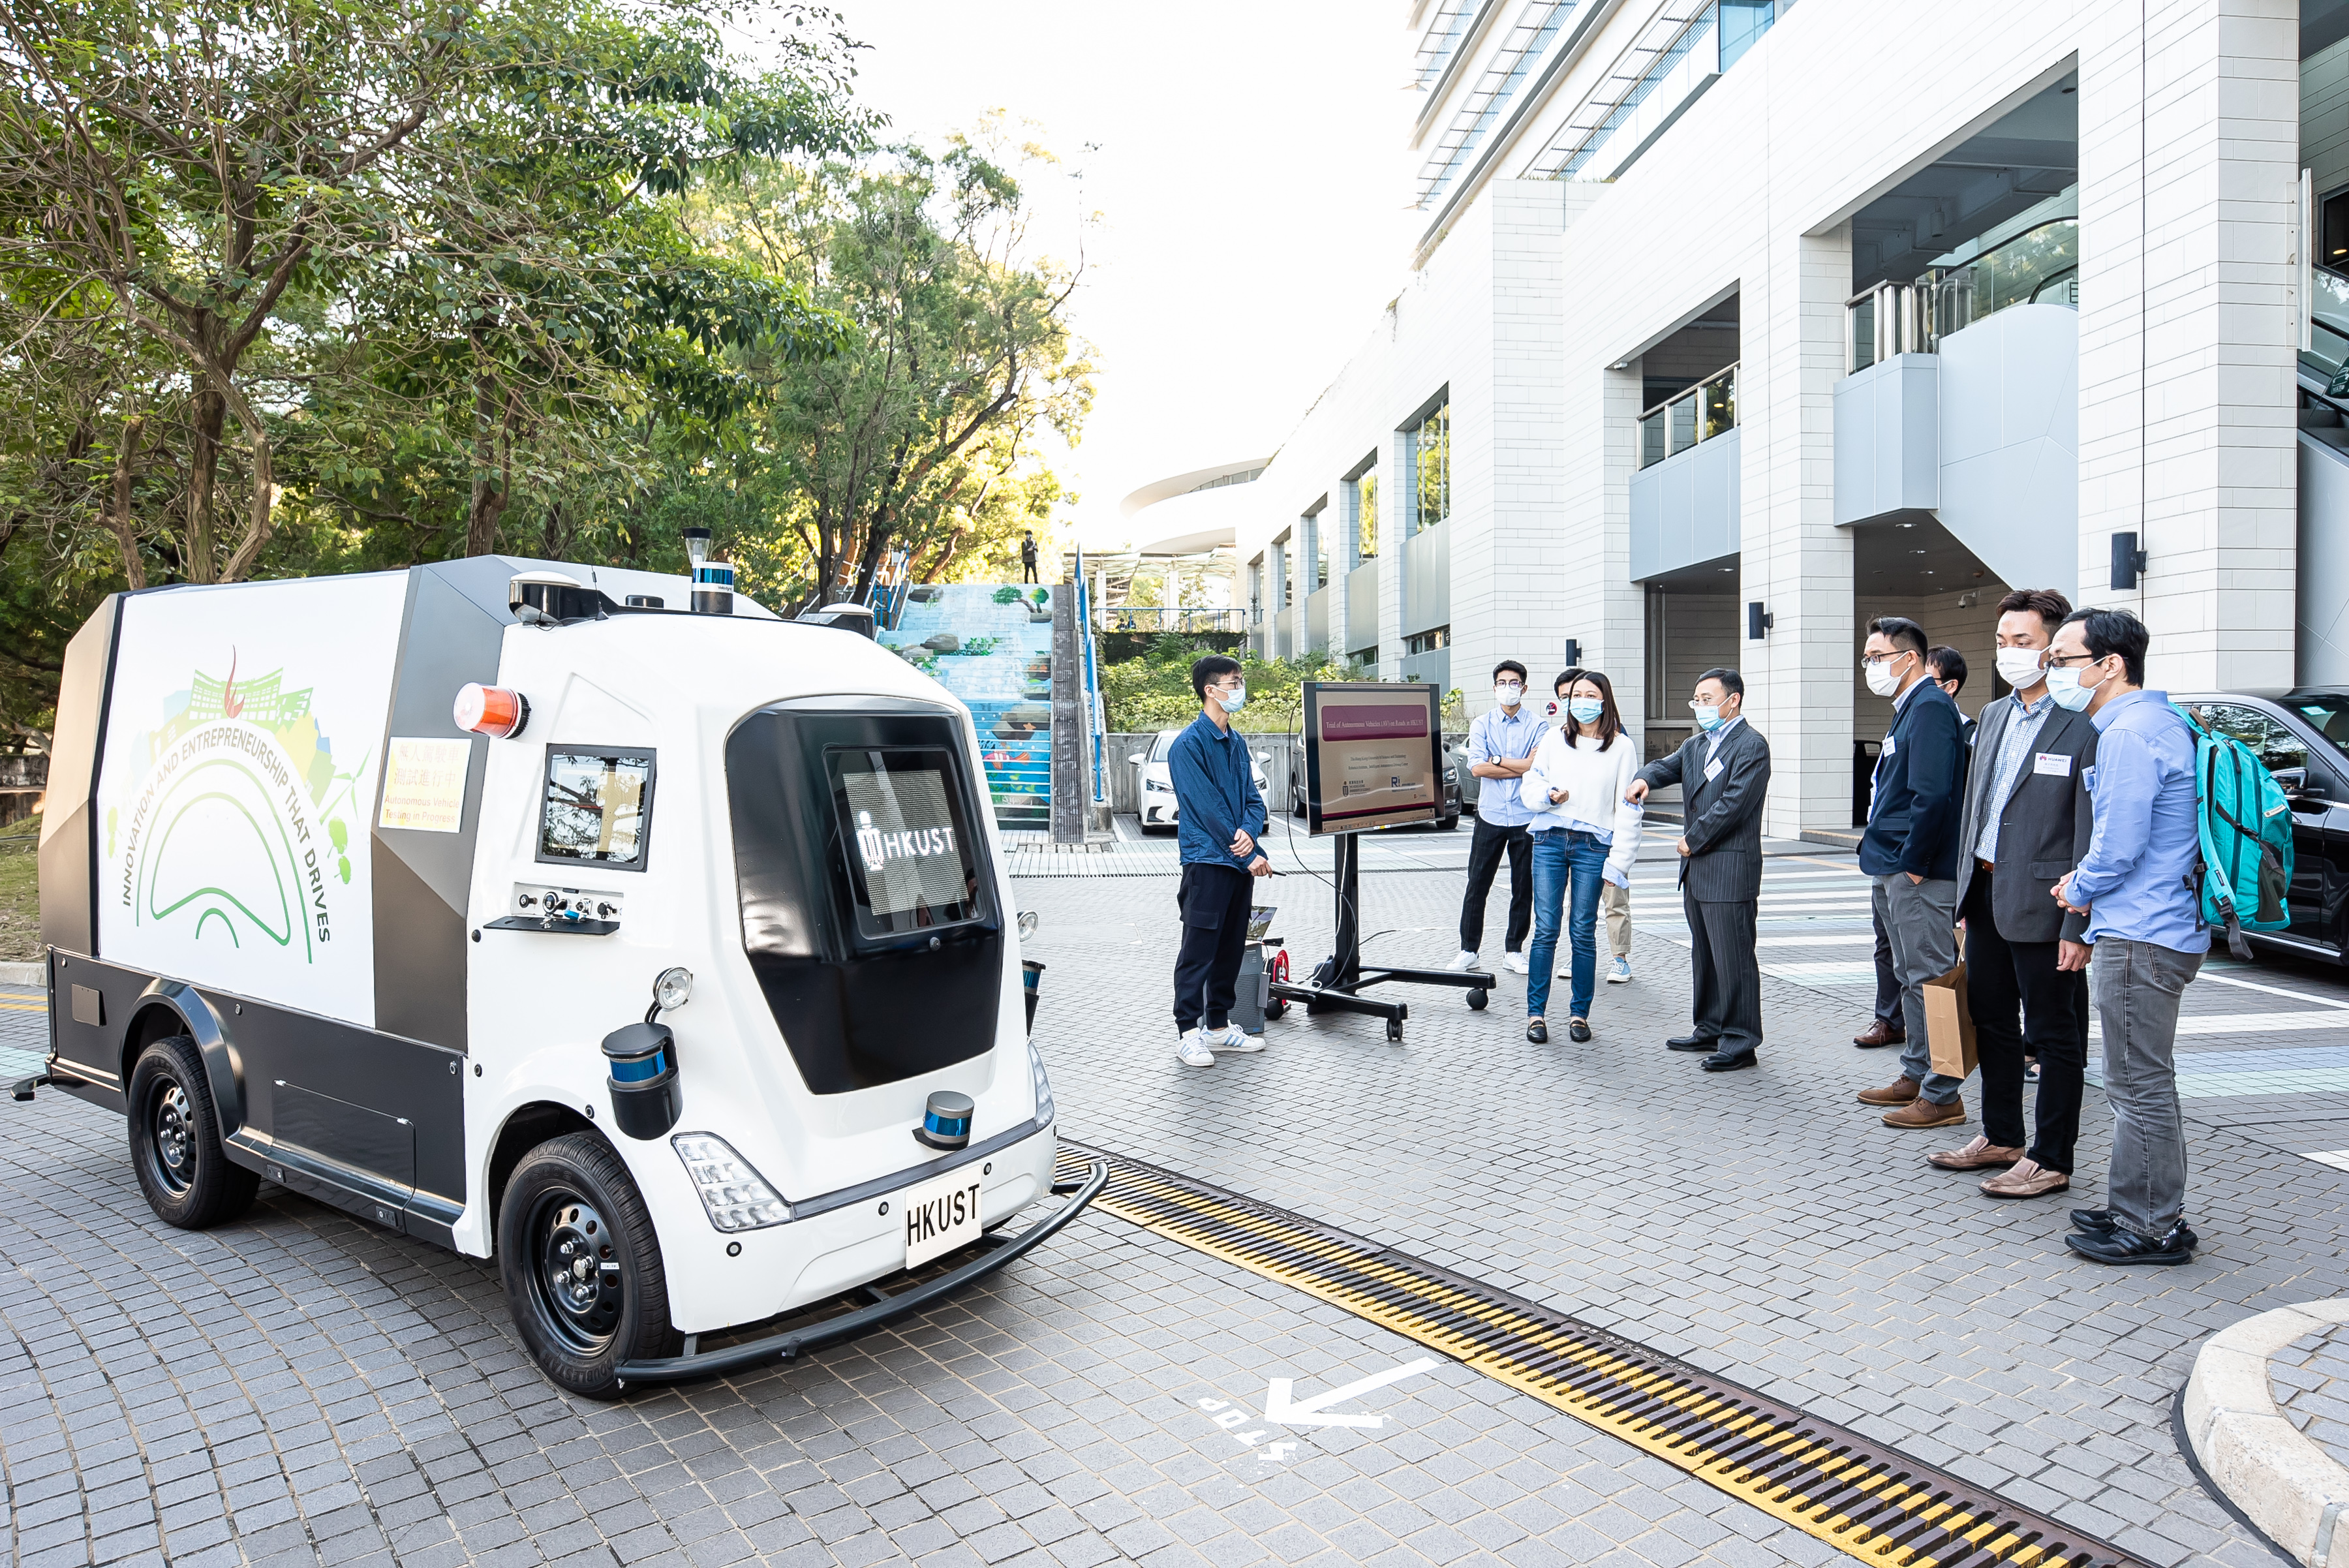
\includegraphics[width=0.9\columnwidth]{figure/pqe/hercules.jpg}
    \caption{The first autonomous vehicle (AV) trial without an operator on board in Hong Kong commenced in late 2020 on the HKUST Clearwater Bay Campus. The AV, designed by Prof. Ming Liu (ECE, Director of HKUST’s Intelligent Autonomous Driving Centre) and his team of students, is one of the many innovative initiatives to fight against the COVID-19 pandemic as the AV can make deliveries that limit human-to-human contact.}
    \label{fig:Hercules}
 \end{figure}

 \begin{figure}[!ht]
    \centering
    \begin{subfigure}{0.45\textwidth}
        \centering
        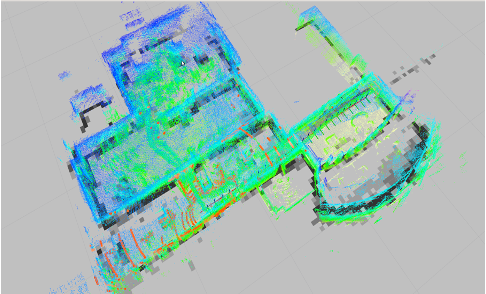
\includegraphics[width=6.5cm, height=4.5cm]{figure/pqe/pointcloudmap.png}
        \caption{A point cloud map of the second floor, HKUST CYT constructed by A-LOAM}
    \end{subfigure}
    \centering
    \begin{subfigure}{0.45\textwidth}
        \centering
        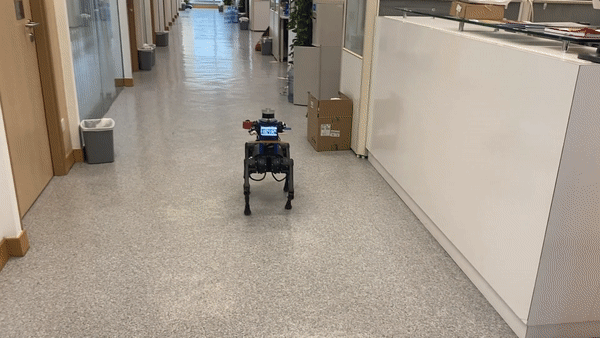
\includegraphics[width=6.5cm, height=4.5cm]{figure/pqe/quadruped.png}
        \caption{A capture of localization on quadruped robot in an indoor office environment.}
    \end{subfigure}
    \caption{Mapping and Localization of Quadruped Robot}
    \label{fig:quadruped}
 \end{figure}

 \begin{figure}[!ht]
    \centering
    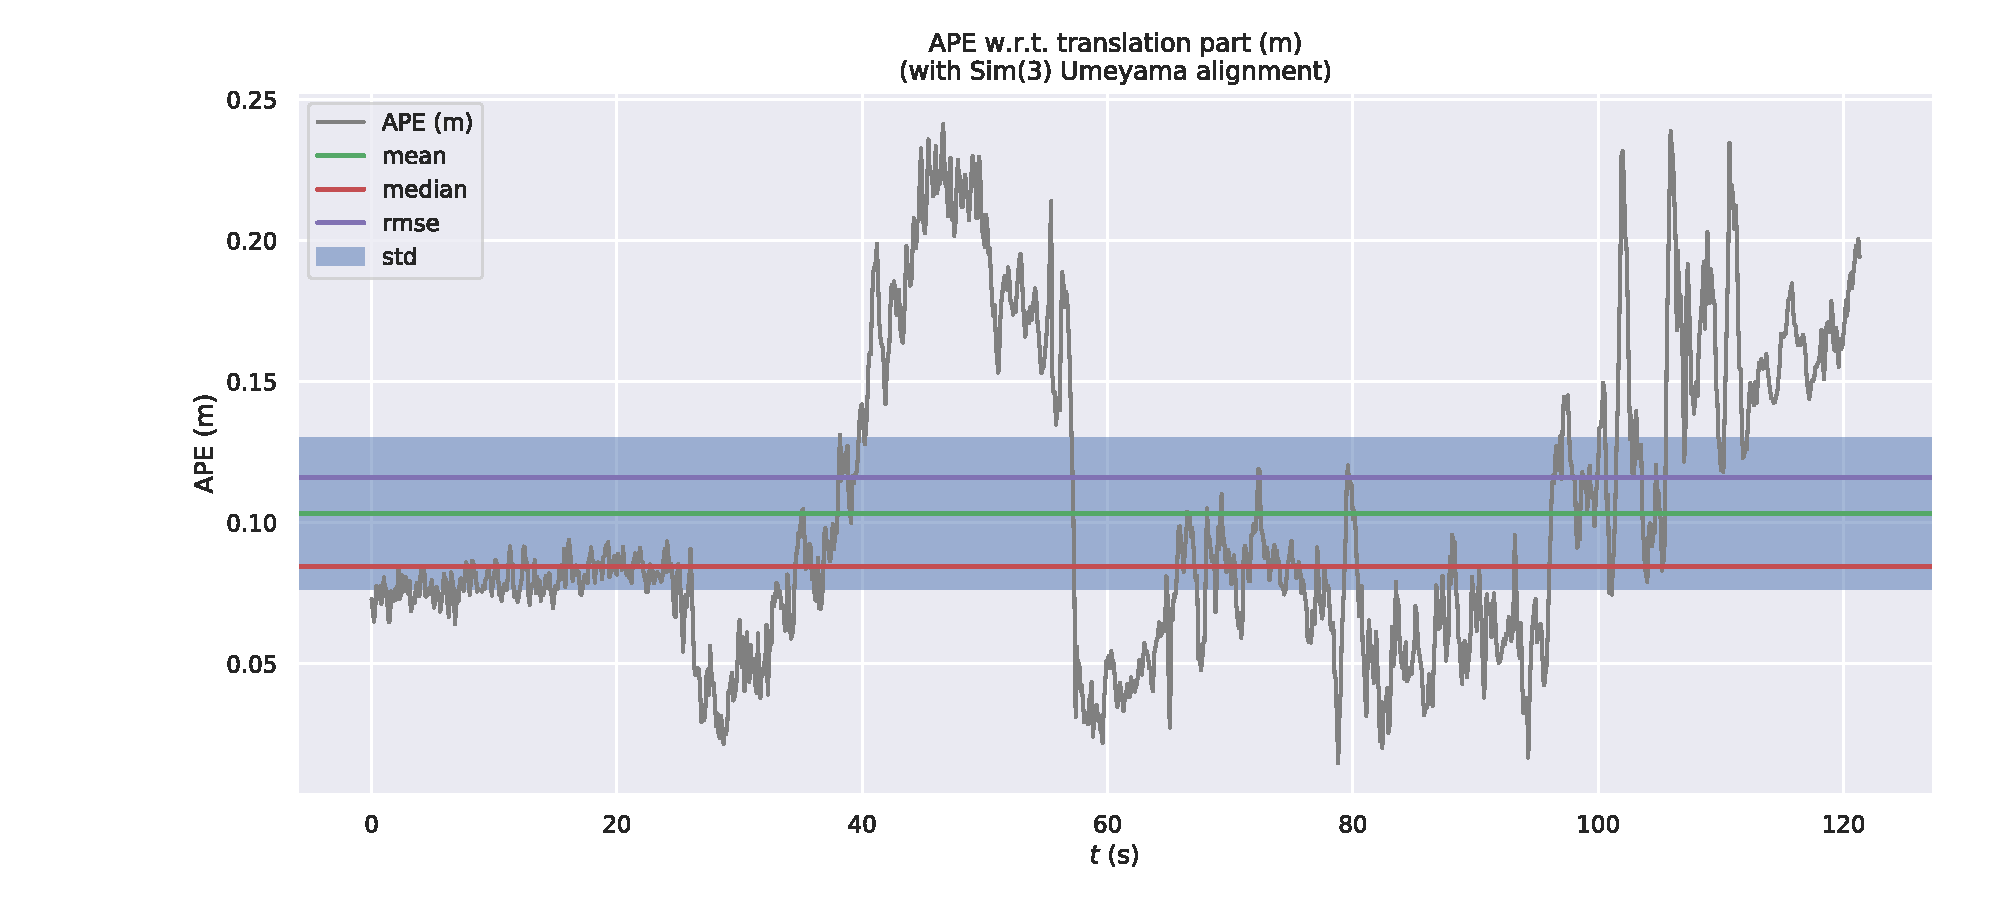
\includegraphics[width=\columnwidth]{figure/pqe/lio2.pdf}
    \caption{Qualitity evaluation result of localization accuracy in the indoor office environment.}
    \label{localizationeva}
 \end{figure}
 \begin{figure}[!ht]
    \centering
    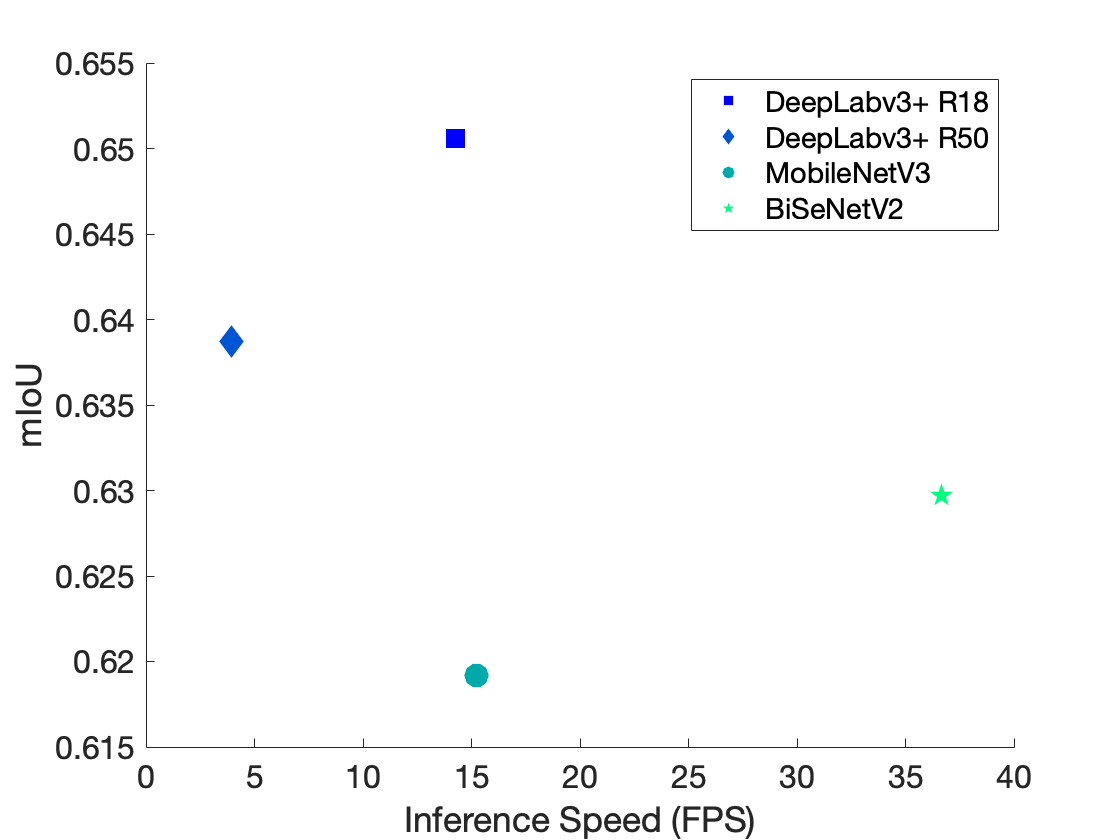
\includegraphics[width=0.75\columnwidth]{figure/pqe/Trade-off.png}
    \caption{The trade-off evaluation between inference speed and segmentation mean Intersection over Union (mIoU) for state-of-the-art segmentation network\cite{yu2021bisenet,howard2019searching,chen2018encoder} }
    \label{cross-evaluation}
 \end{figure}

 \begin{figure}[!ht]
    \centering
    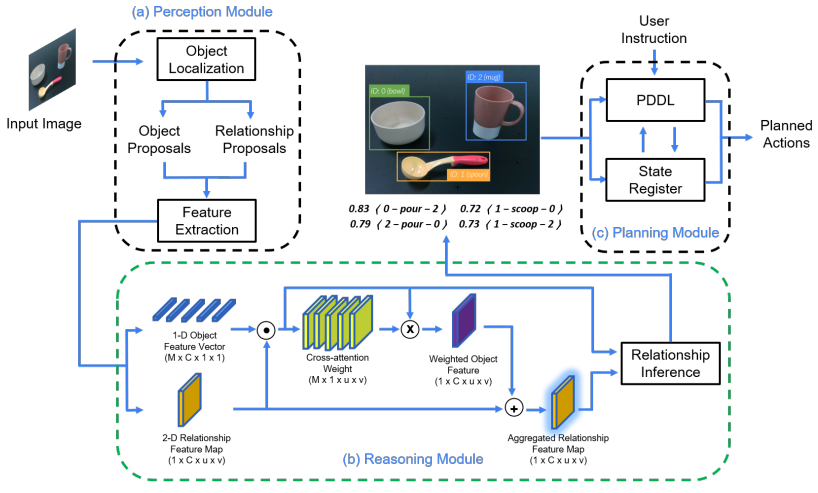
\includegraphics[width=0.9\columnwidth]{figure/pqe/pipeline_relationship.png}
    \caption{The whole pipeline of relationship-oriented semantic scene understanding. Overview: the pipeline first uses (a) perception module to localize all possible object and relationship proposals. A novel relationship-attention
    the mechanism in the (b) reasoning module is then deployed to aggregate the relationship feature map and infer the relationships along with their probabilities.
    Finally, the output from the last step seeds the (c) planning module for goal-oriented, multi-step manipulation task planning according to user instructions. }
    \label{fig:pipeline_relationship}
 \end{figure}

 \begin{figure}[!ht]
    \centering
    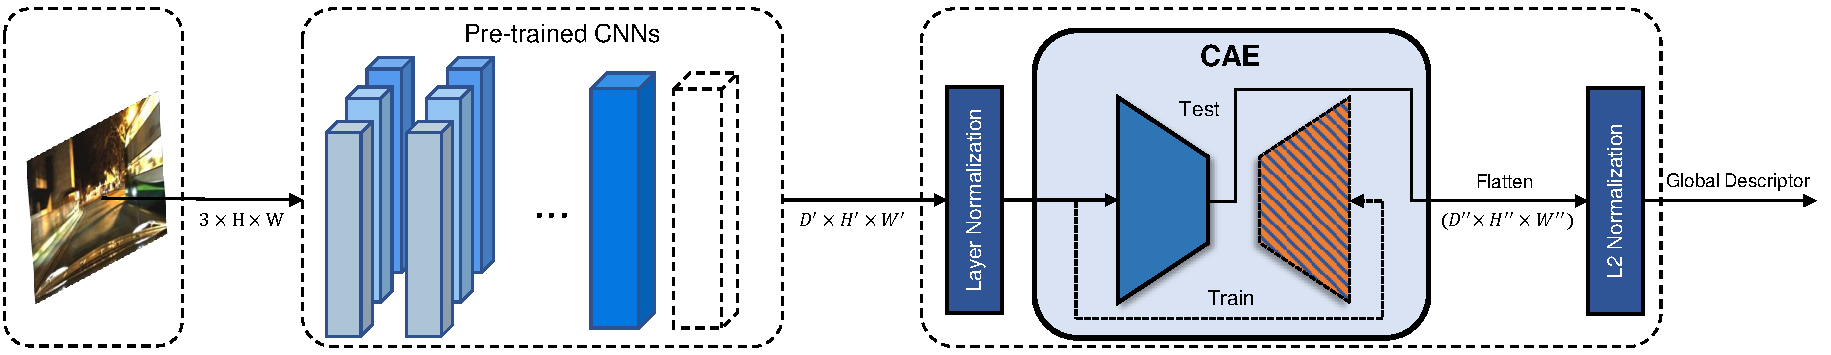
\includegraphics[width=\columnwidth]{figure/pqe/approach.pdf}
	\caption{The detailed pipeline of \cite{ye2022condition}. Given an image with $3\times{H}\times{W}$, CNNs  extract the local feature map $X_i$ with $D^{'}\times{H^{'}}\times{W^{'}}$. The CNNs are classification pre-trained or VPR-trained, e.g. AlexNet, VGG16. Both are cut at the last convolutional layer (conv5), before ReLU. In the training time, CAE is trained unsupervised by a reconstruction loss. In the test time, the decoder part of CAE is not involved and the encoder part is kept to compress the normalized feature map and produce a low-dimensional global descriptor with $D^{''}\times{H^{''}}\times{W^{''}}$. The global descriptor is then flattened and L2 normalized.}
    \label{fig:approach_VPR}
 \end{figure}



\begin{figure}[!ht]
\centering
\begin{subfigure}{0.4\textwidth}
    \centering
    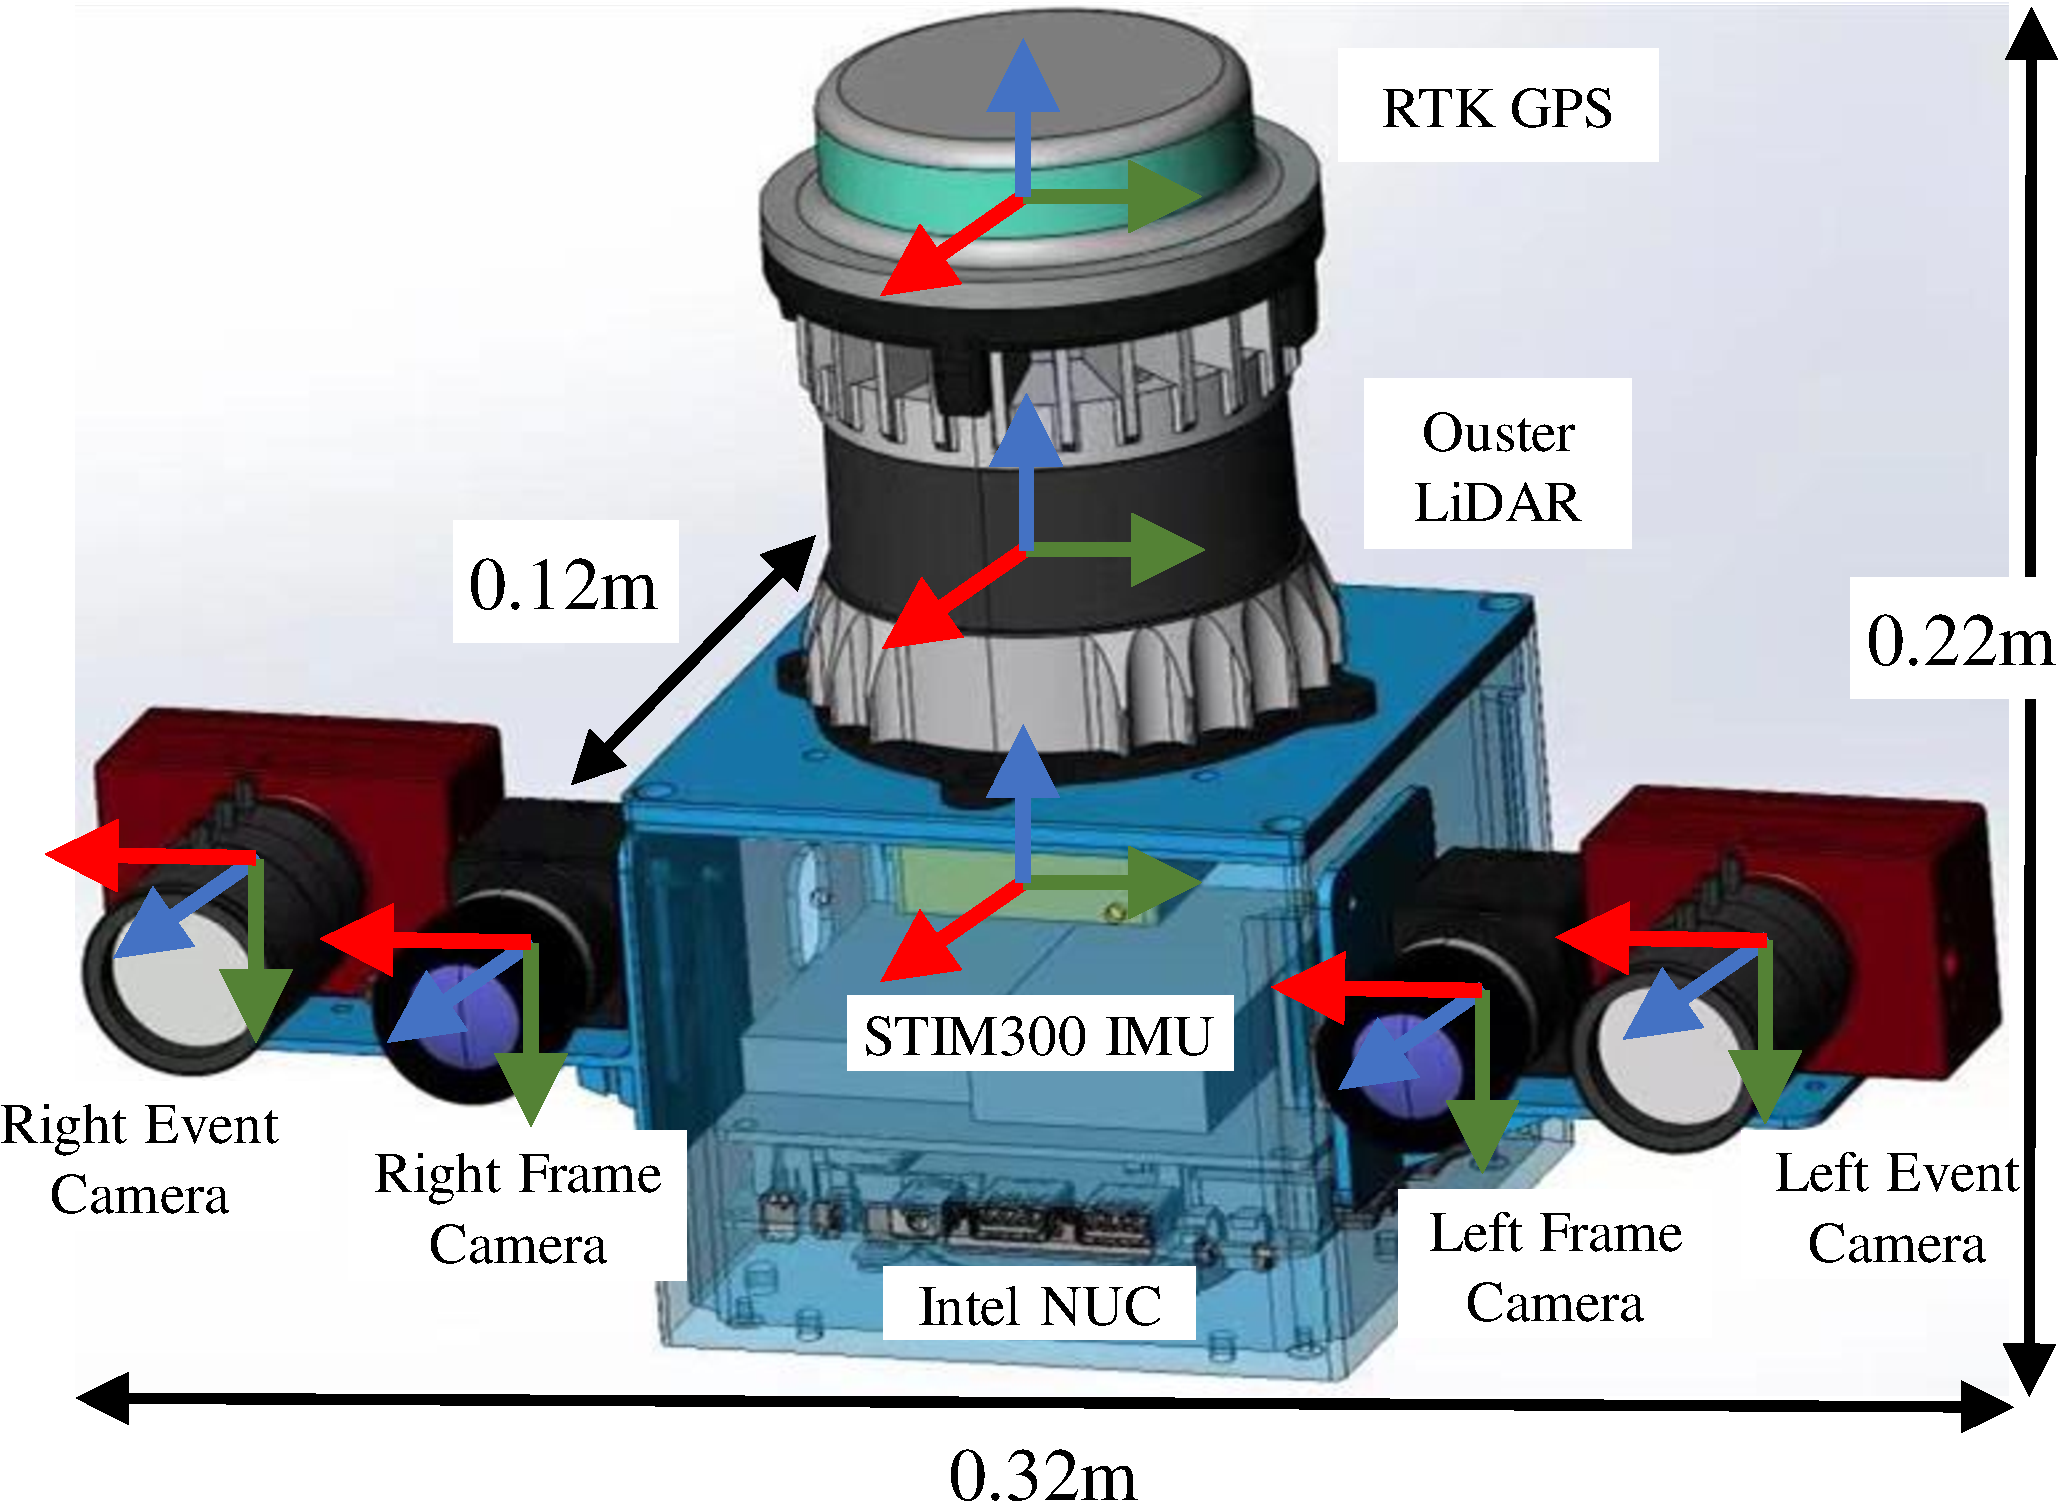
\includegraphics[width=0.8\textwidth, height=5cm]{figure/pqe/methodology/handheld_device-crop.pdf}
    \caption{}
    % \caption{A point cloud map of the second floor, HKUST CYT constructed by A-LOAM}
\end{subfigure}
\centering
\begin{subfigure}{0.4\textwidth}
    \centering
    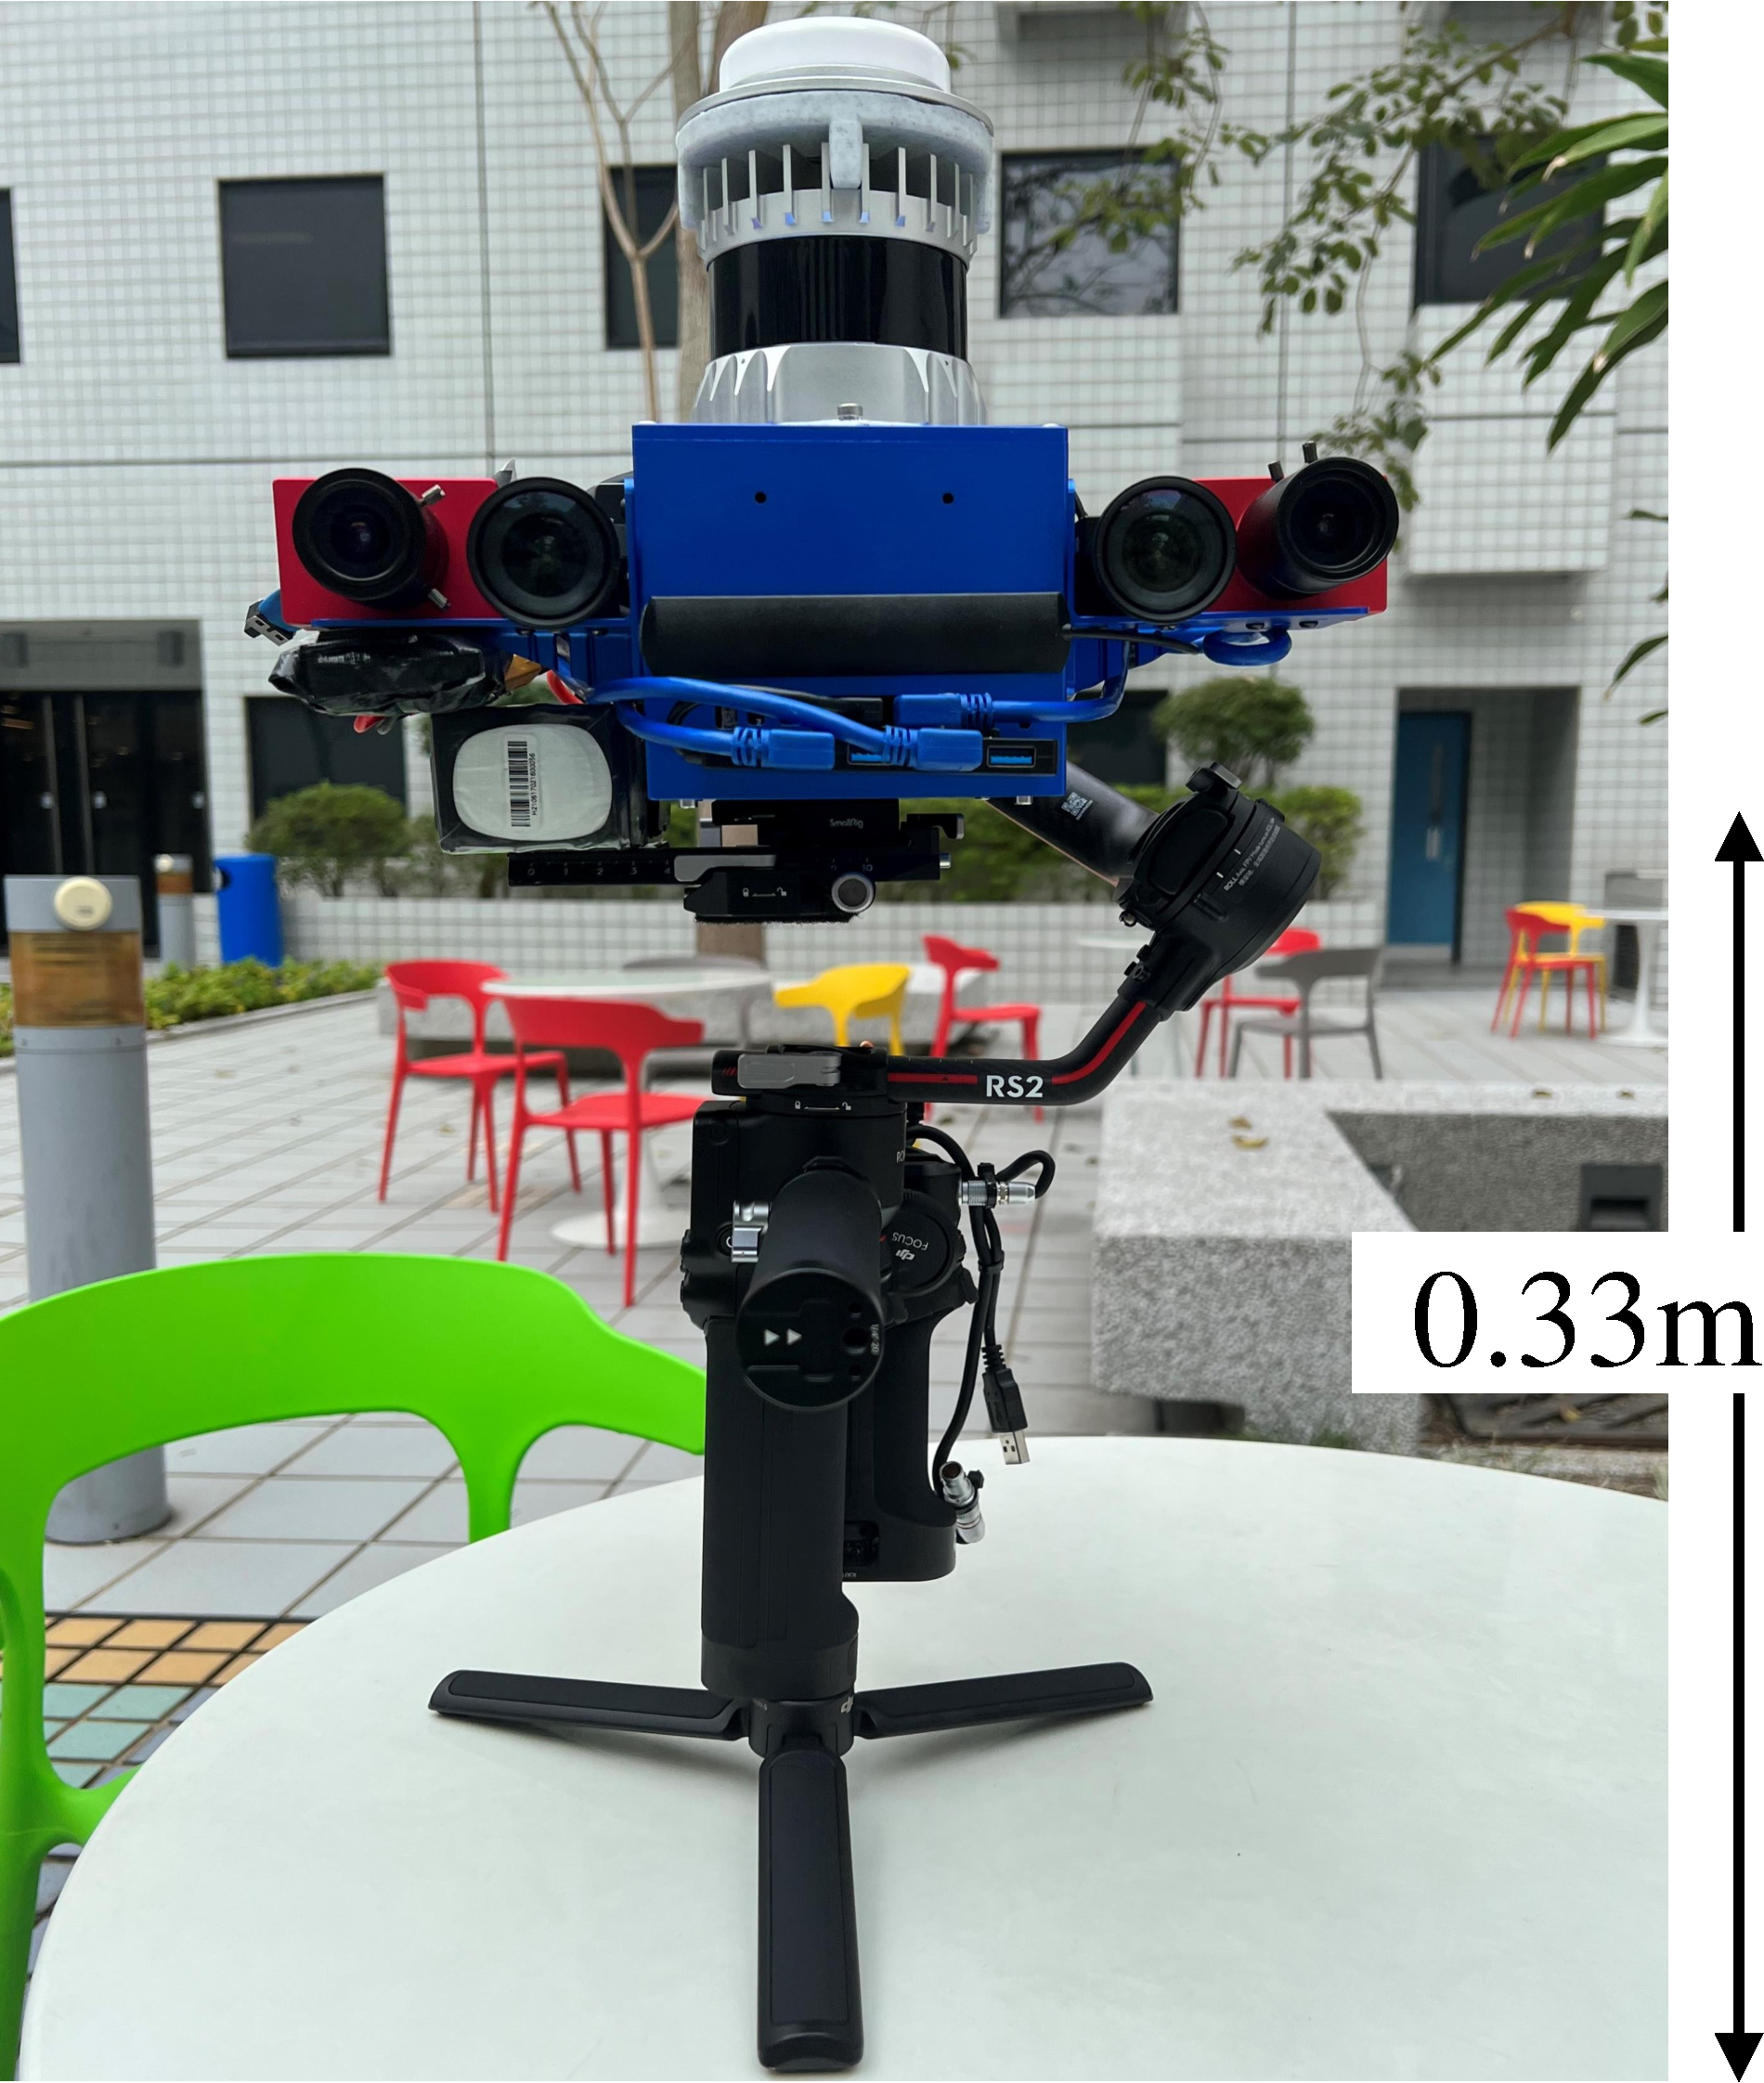
\includegraphics[width=0.8\textwidth, height=5cm]{figure/pqe/methodology/handheld_2-crop.pdf}
    \caption{}
    % \caption{A capture of localization on quadruped robot in an indoor office environment.}
\end{subfigure}
\begin{subfigure}{0.4\textwidth}
    \centering
    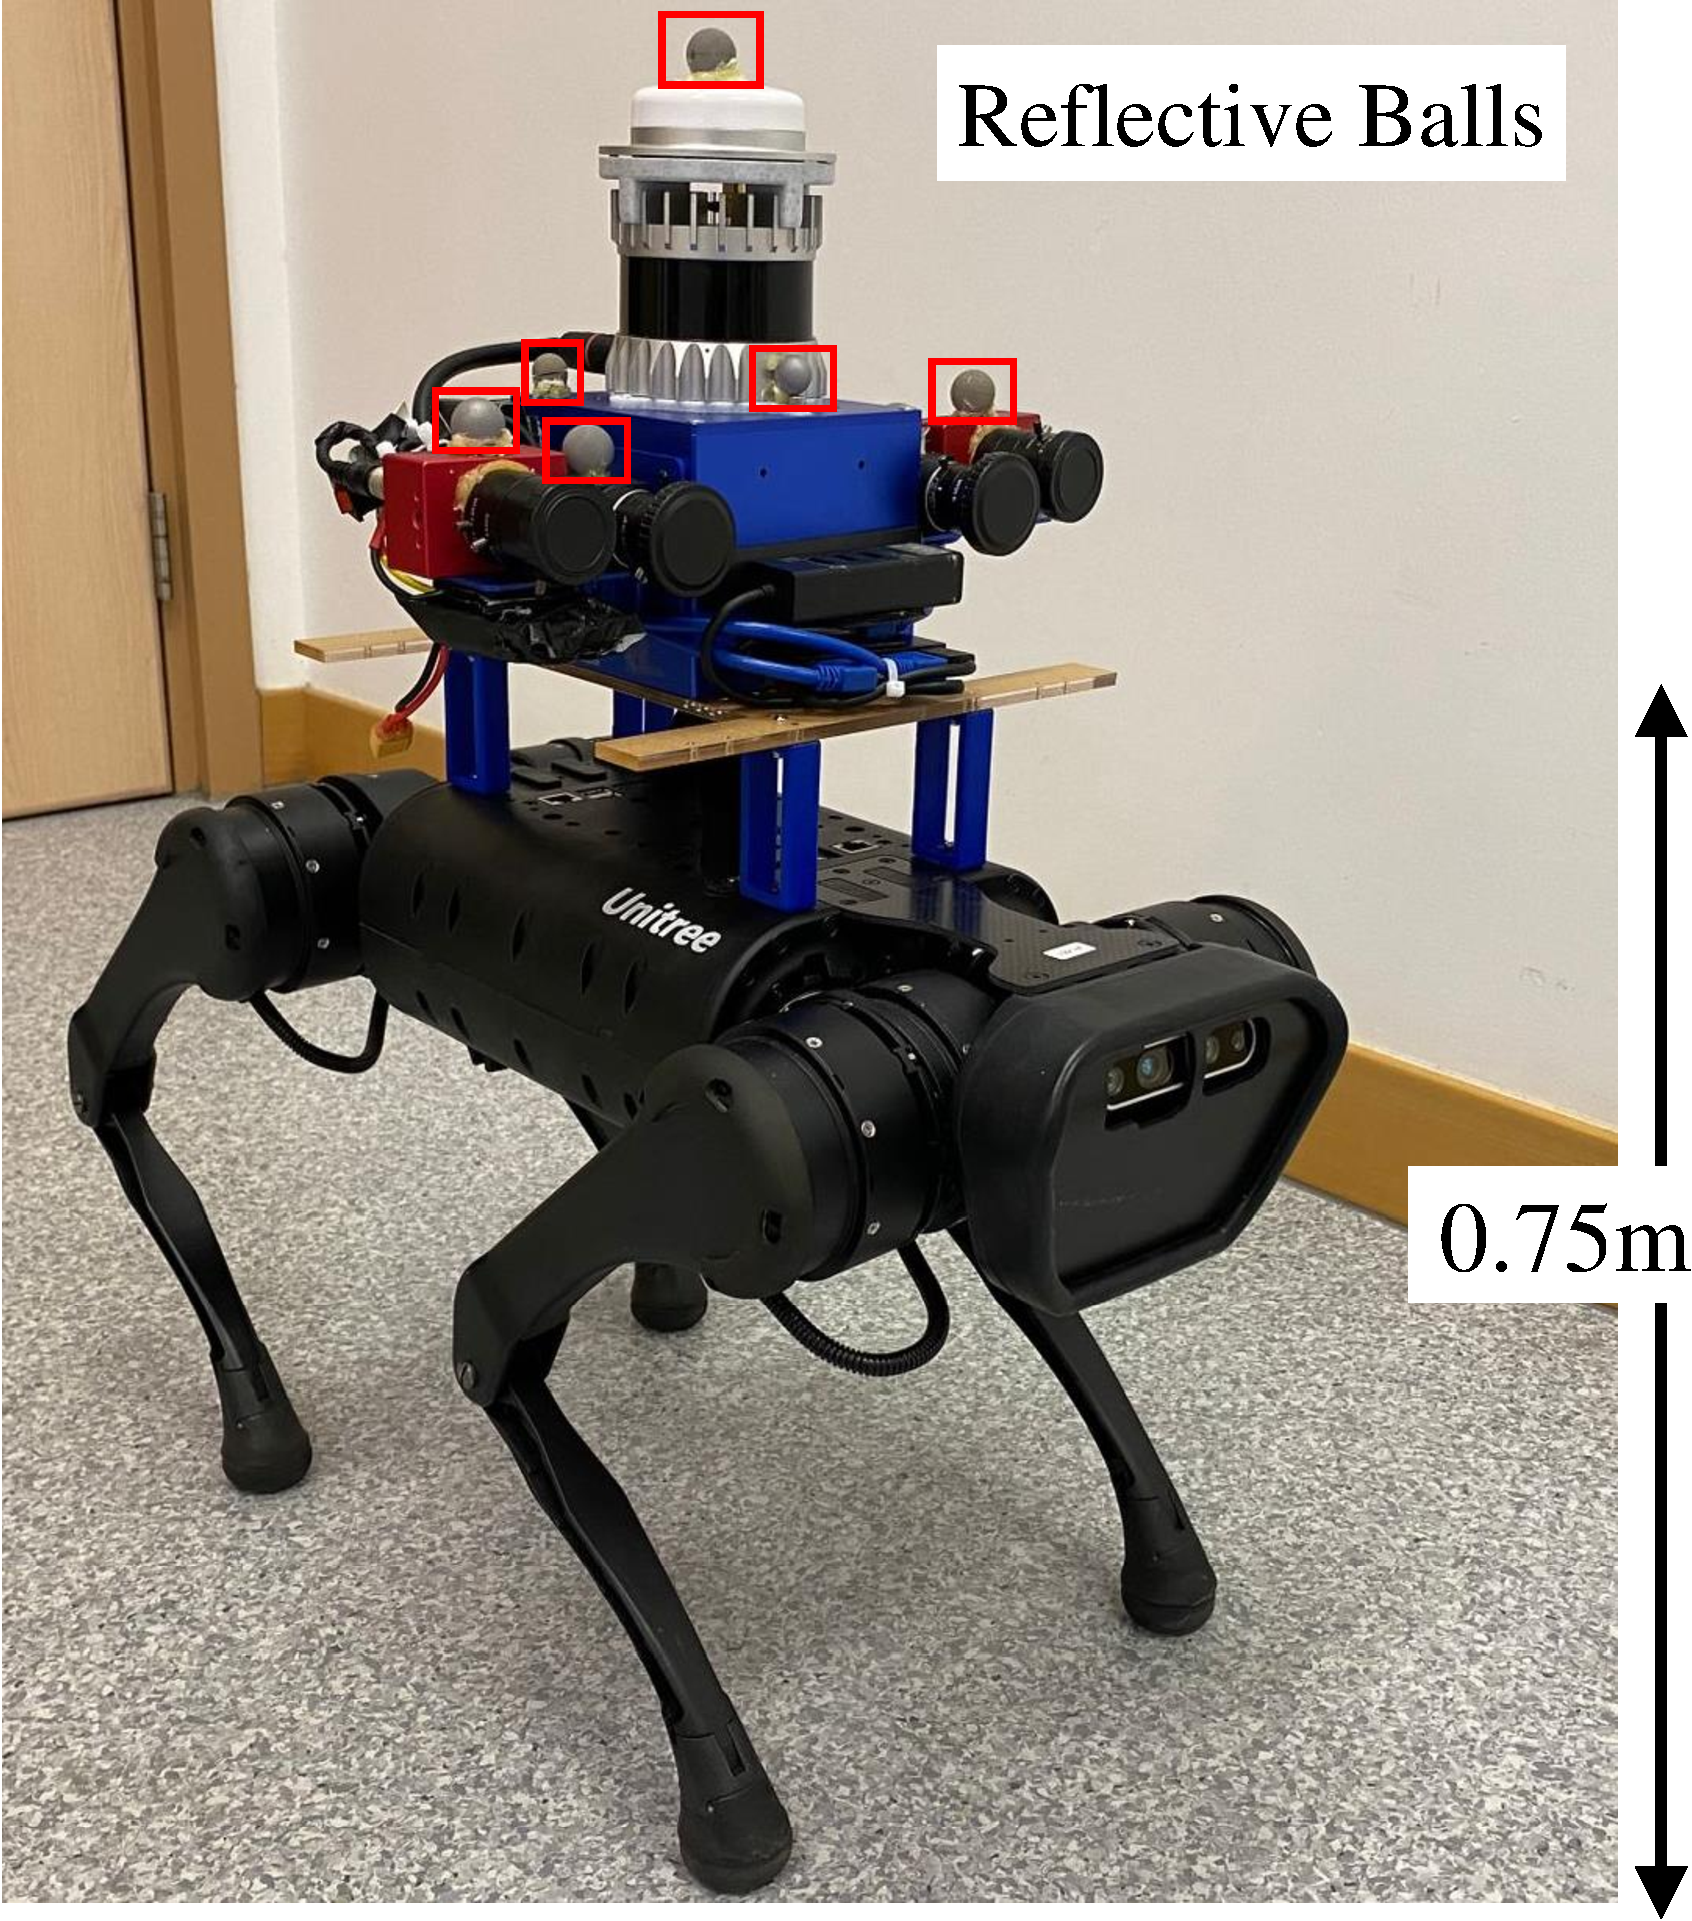
\includegraphics[width=0.8\textwidth, height=5cm]{figure/pqe/methodology/robotdog-crop.pdf}
    \caption{}
    % \caption{A capture of localization on quadruped robot in an indoor office environment.}
\end{subfigure}
\begin{subfigure}{0.4\textwidth}
    \centering
    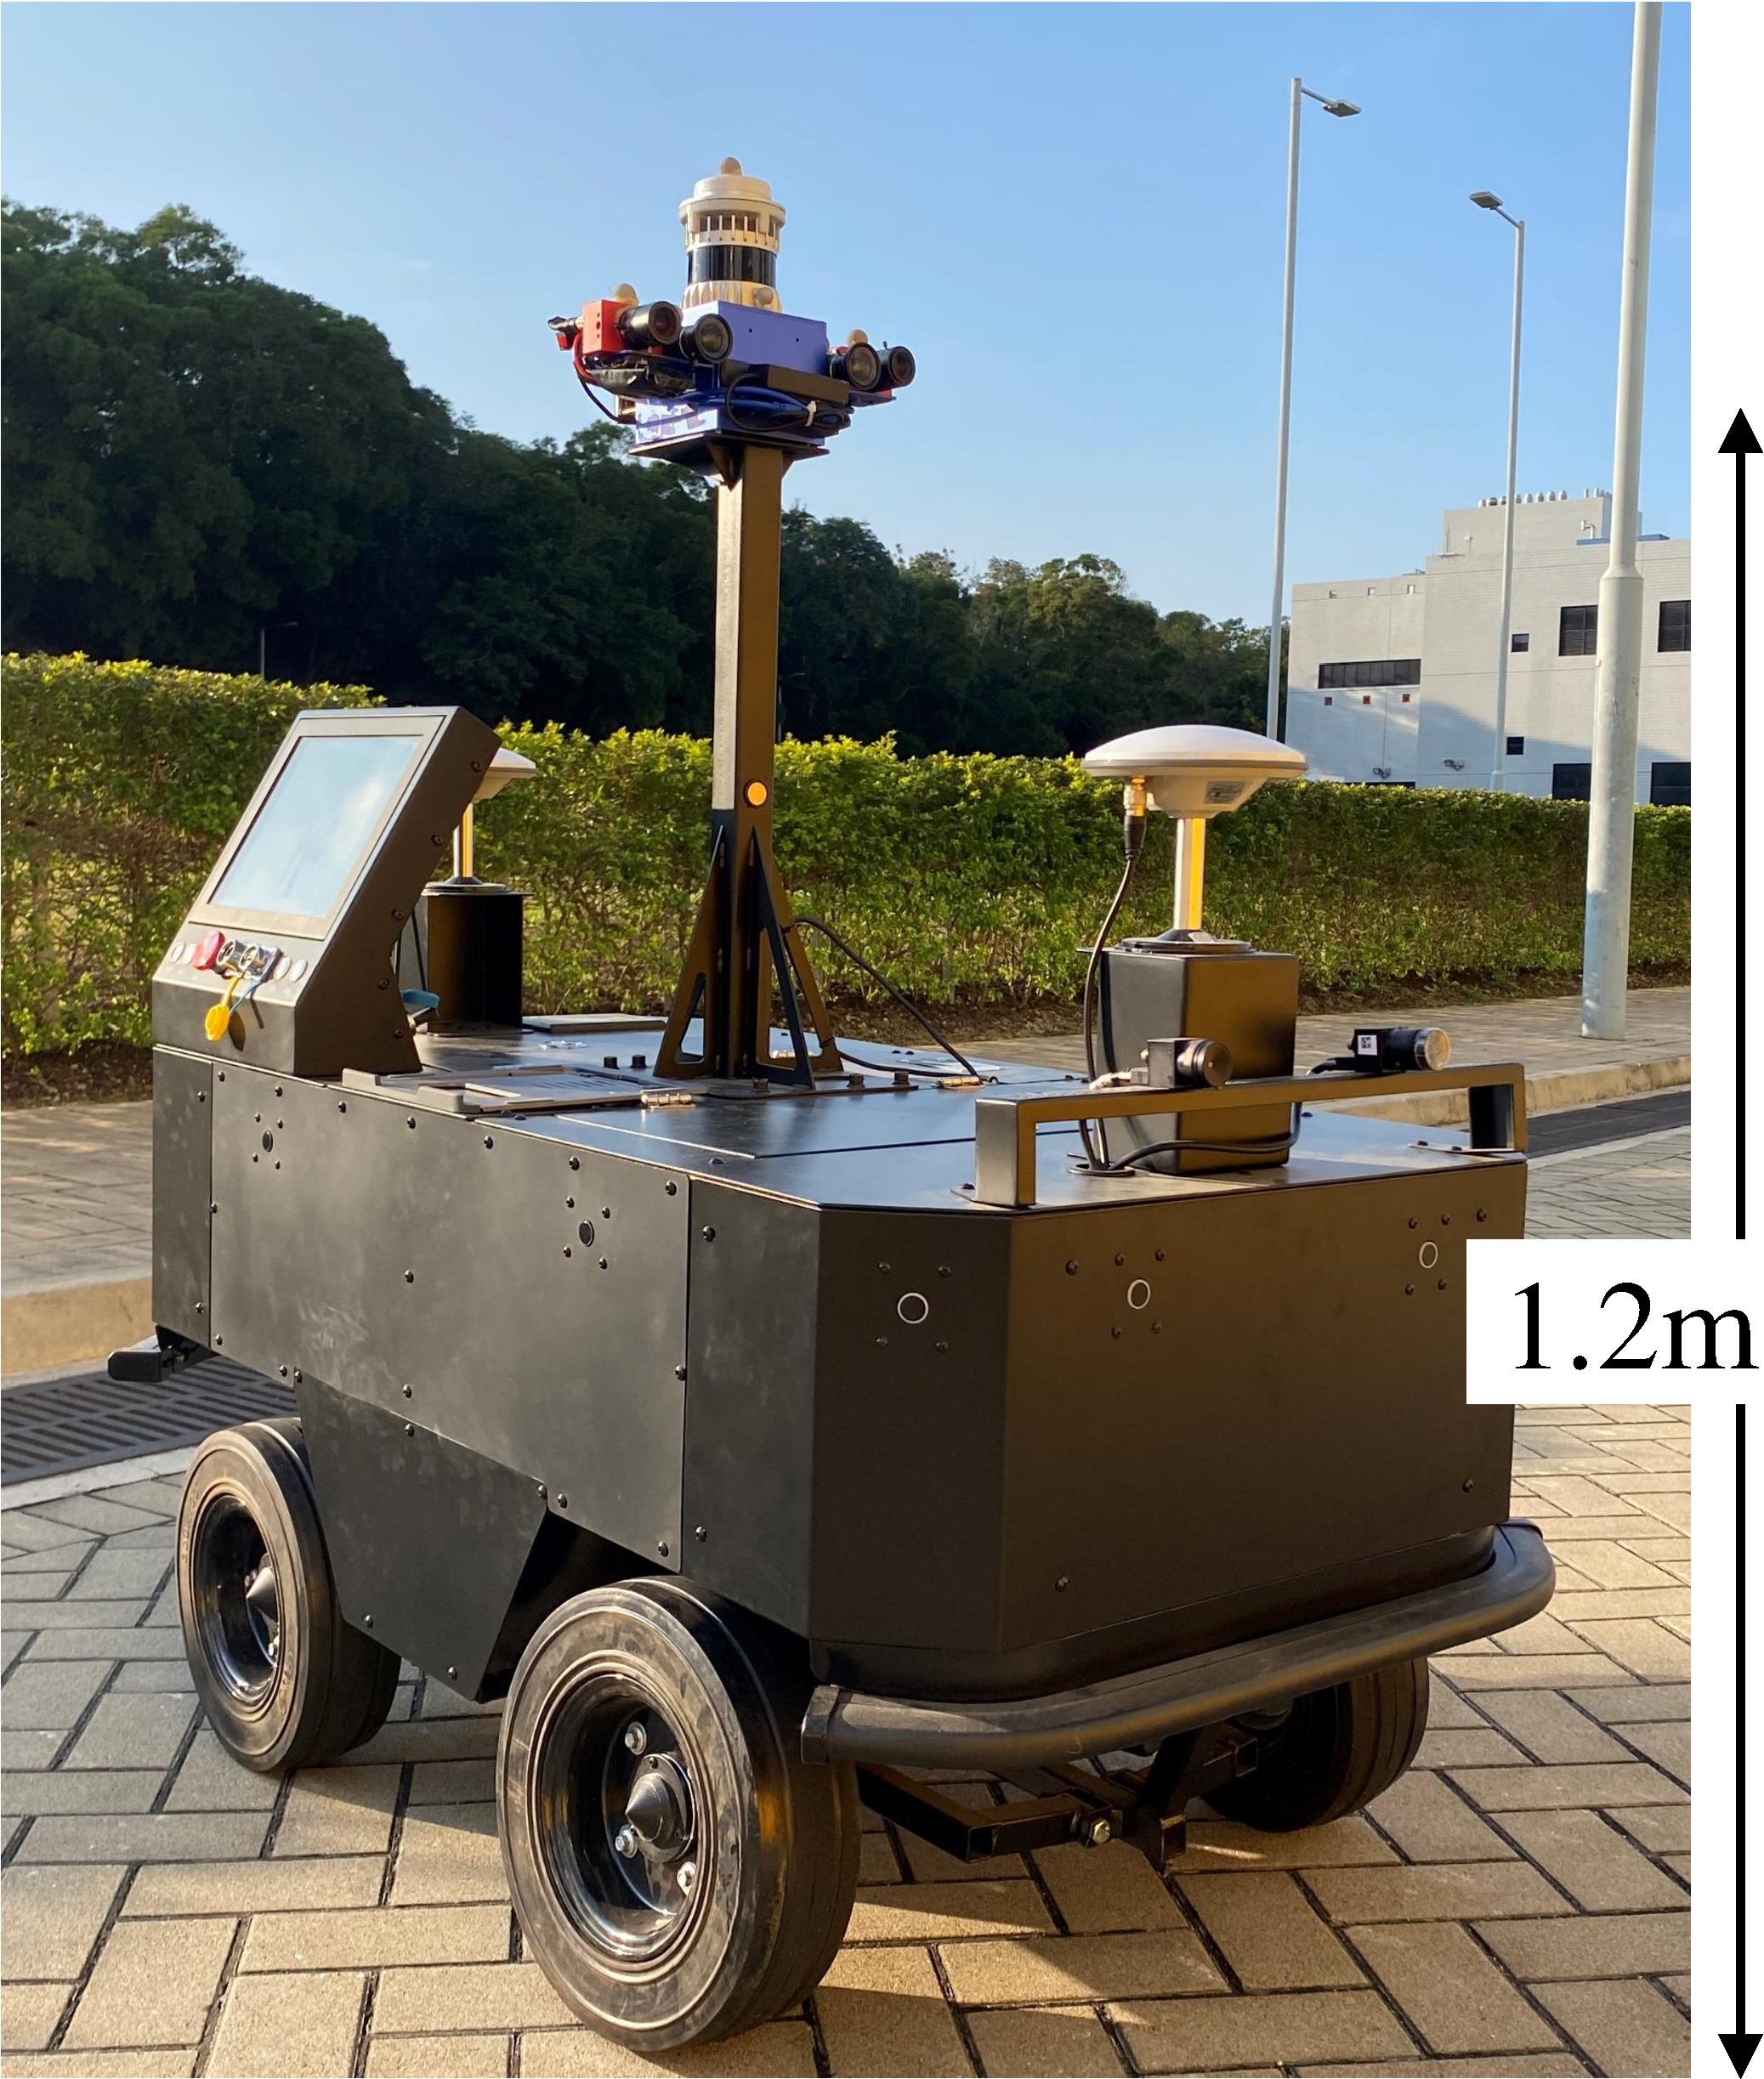
\includegraphics[width=0.8\textwidth, height=5cm]{figure/pqe/methodology/apollo-crop.pdf}
    \caption{}
    % \caption{A capture of localization on quadruped robot in an indoor office environment.}
\end{subfigure}

\caption{The multi-sensor device and data collection platform: 
(a) CAD model of the sensor rig, where axis directions are colored: red: $X$, green: $Y$, blue: $Z$. The sensor rig is rigidly mounted on (b) a gimbal stabilizer, (c) a quadruped robot, and (d) an apollo autonomous vehicle.}
\label{fig:FusionPortable}
\end{figure}
 
 



% \begin{figure}[ht]
% \centering
% \begin{subfigure}
% {\label{fig:sensor_handheld}
% \hspace{0.2cm}
% \centering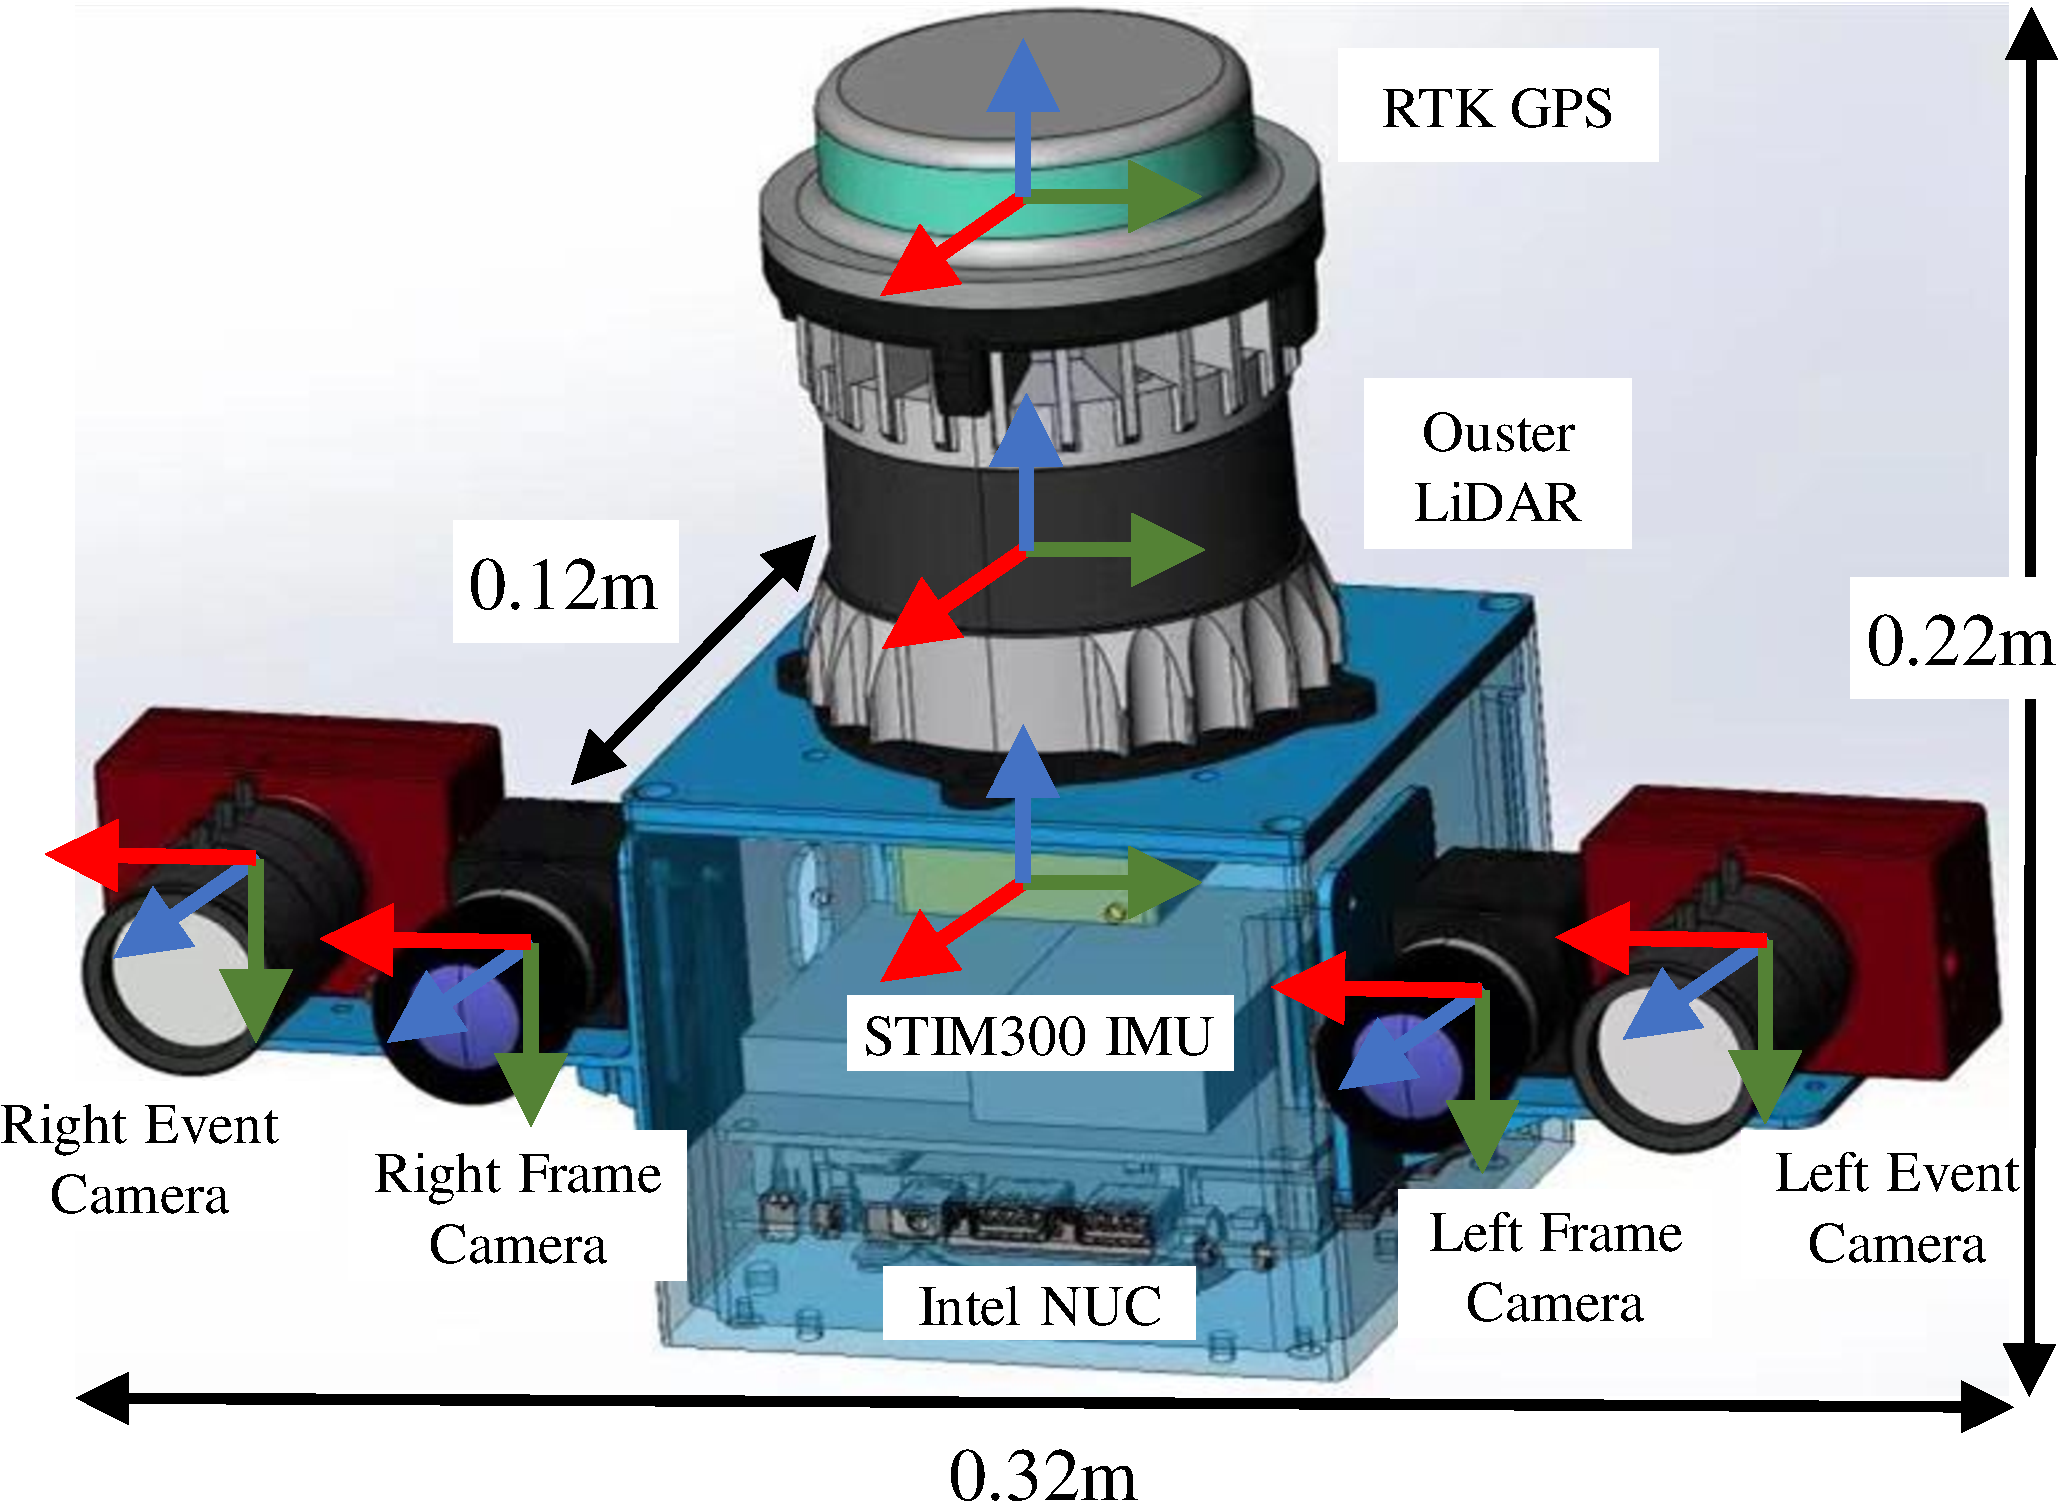
\includegraphics[width=.2746\linewidth]{figure/pqe/methodology/handheld_device-crop.pdf}}
% \end{subfigure}
% \begin{subfigure}{\label{fig:sensor_stab}\centering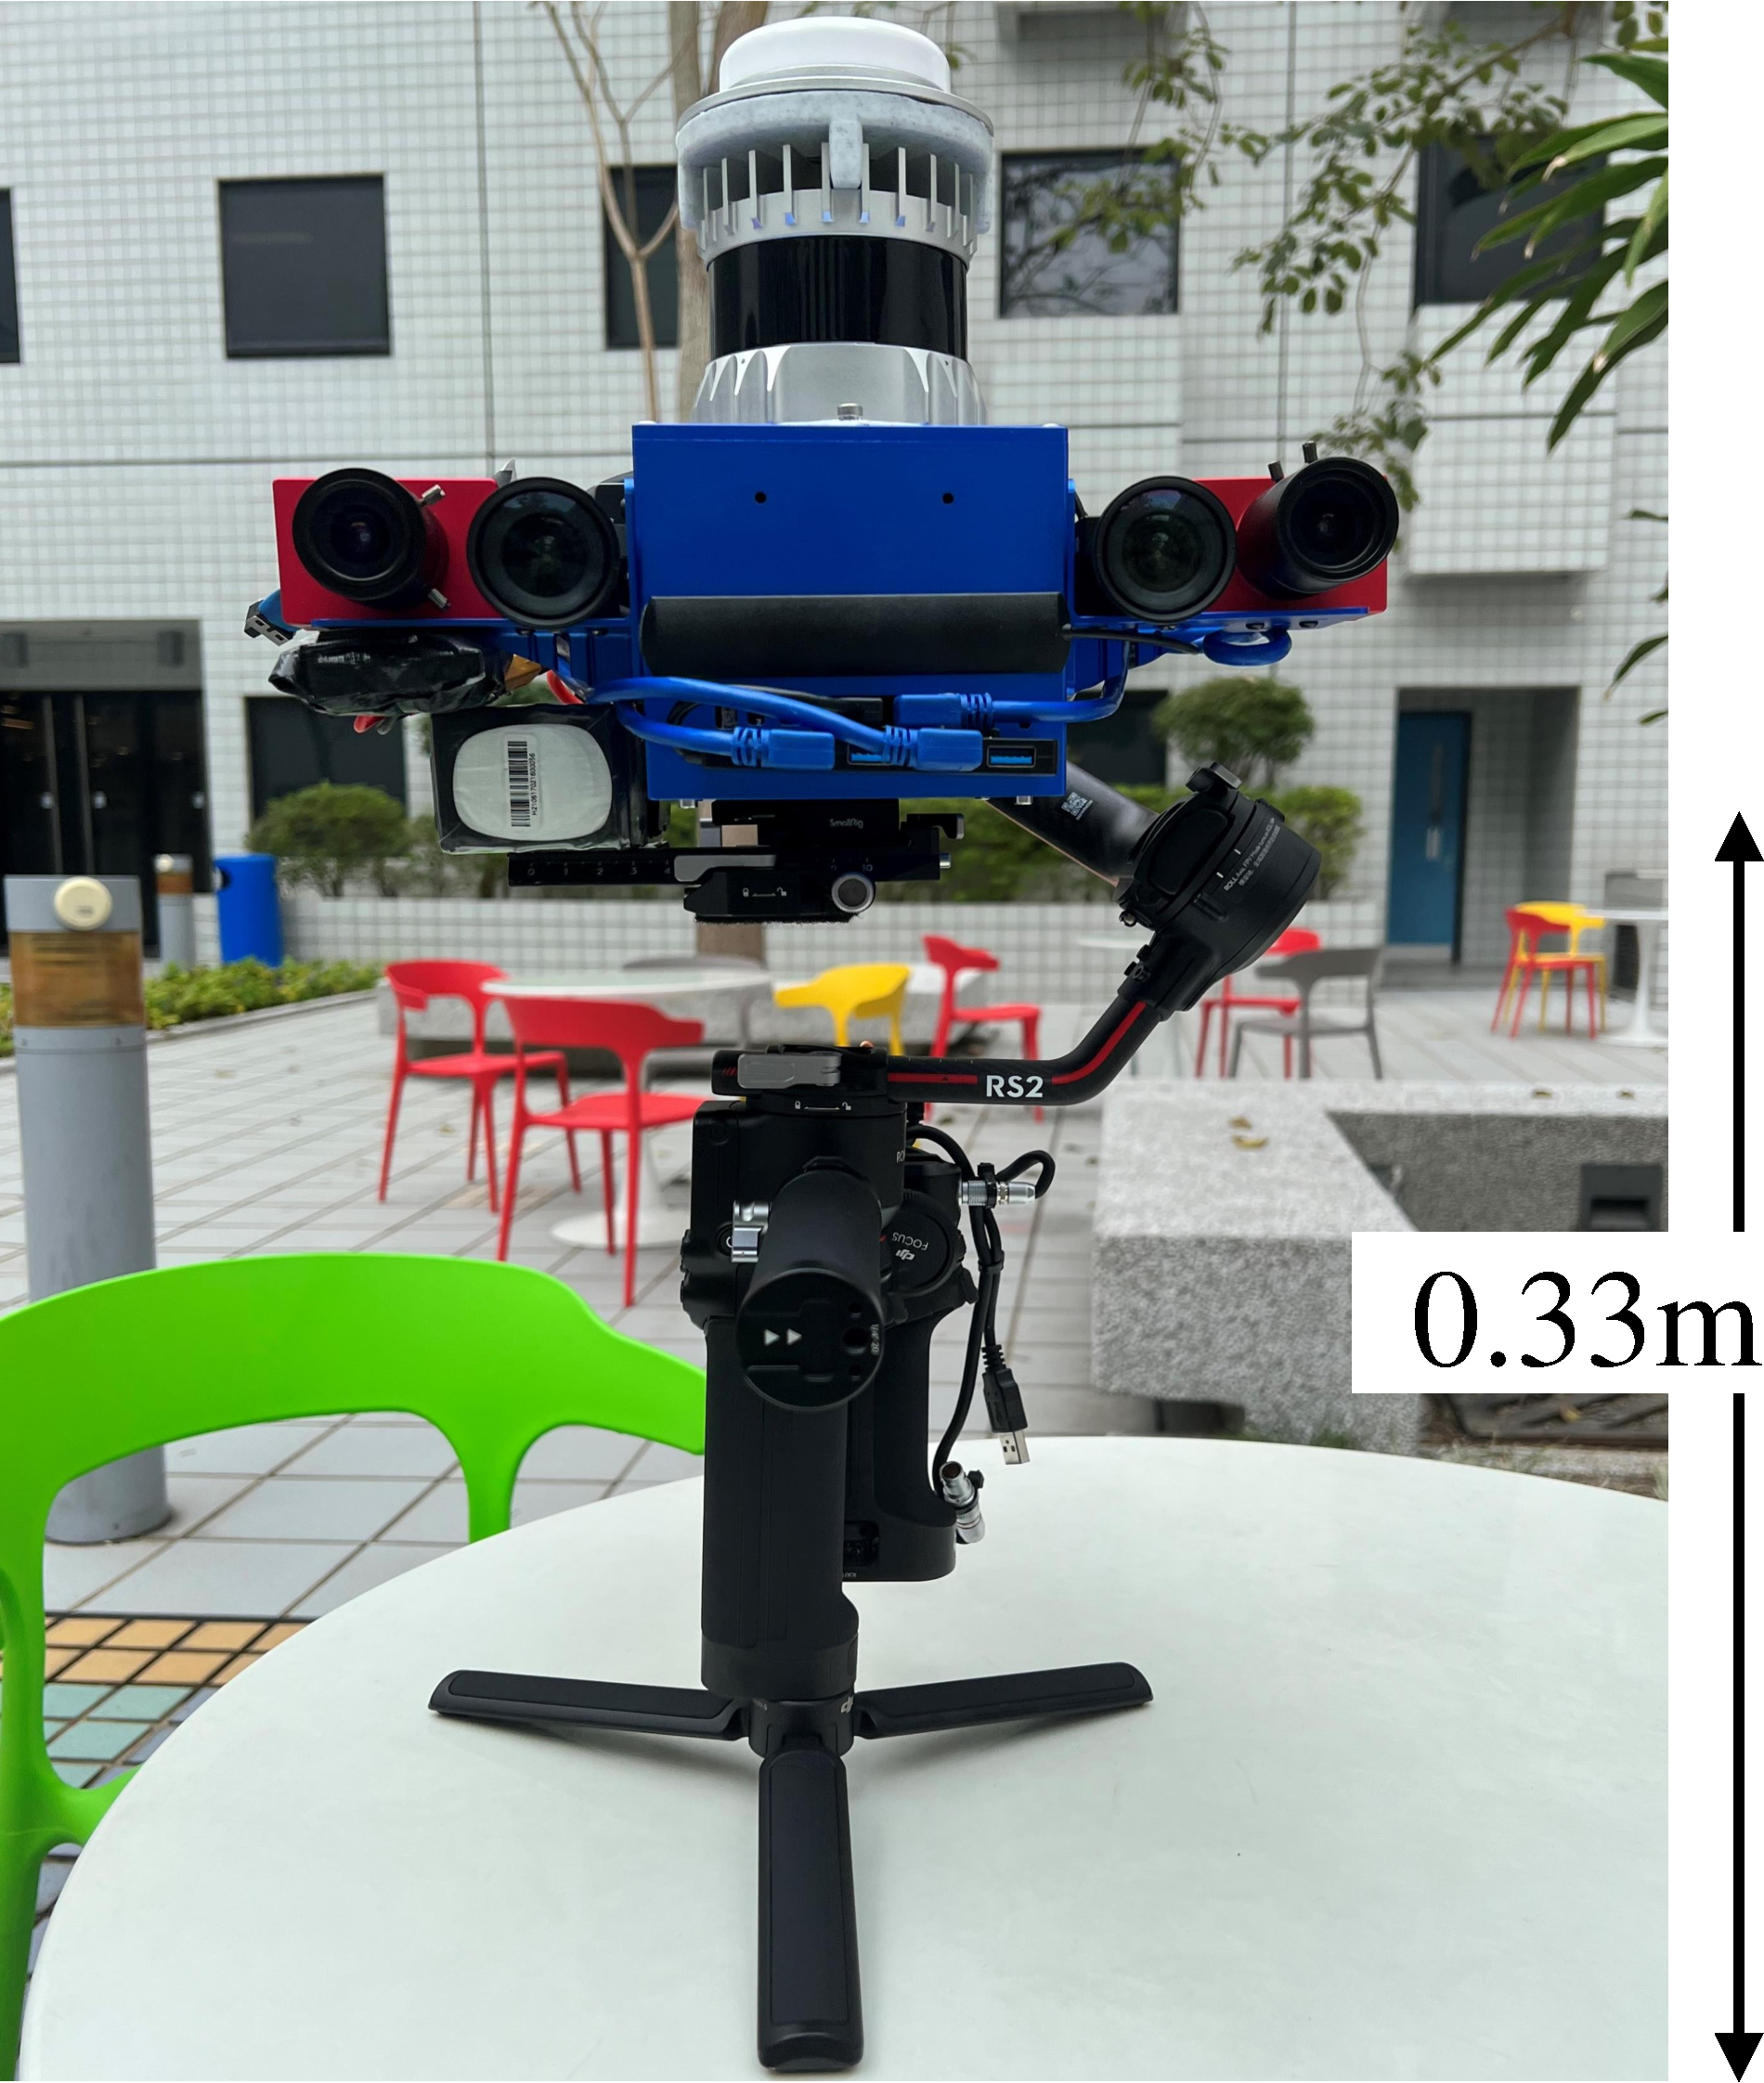
\includegraphics[width=.1701\linewidth]{figure/pqe/methodology/handheld_2-crop.pdf}}
% \end{subfigure}
% \begin{subfigure}{\label{fig:sensor_quadrobot}\centering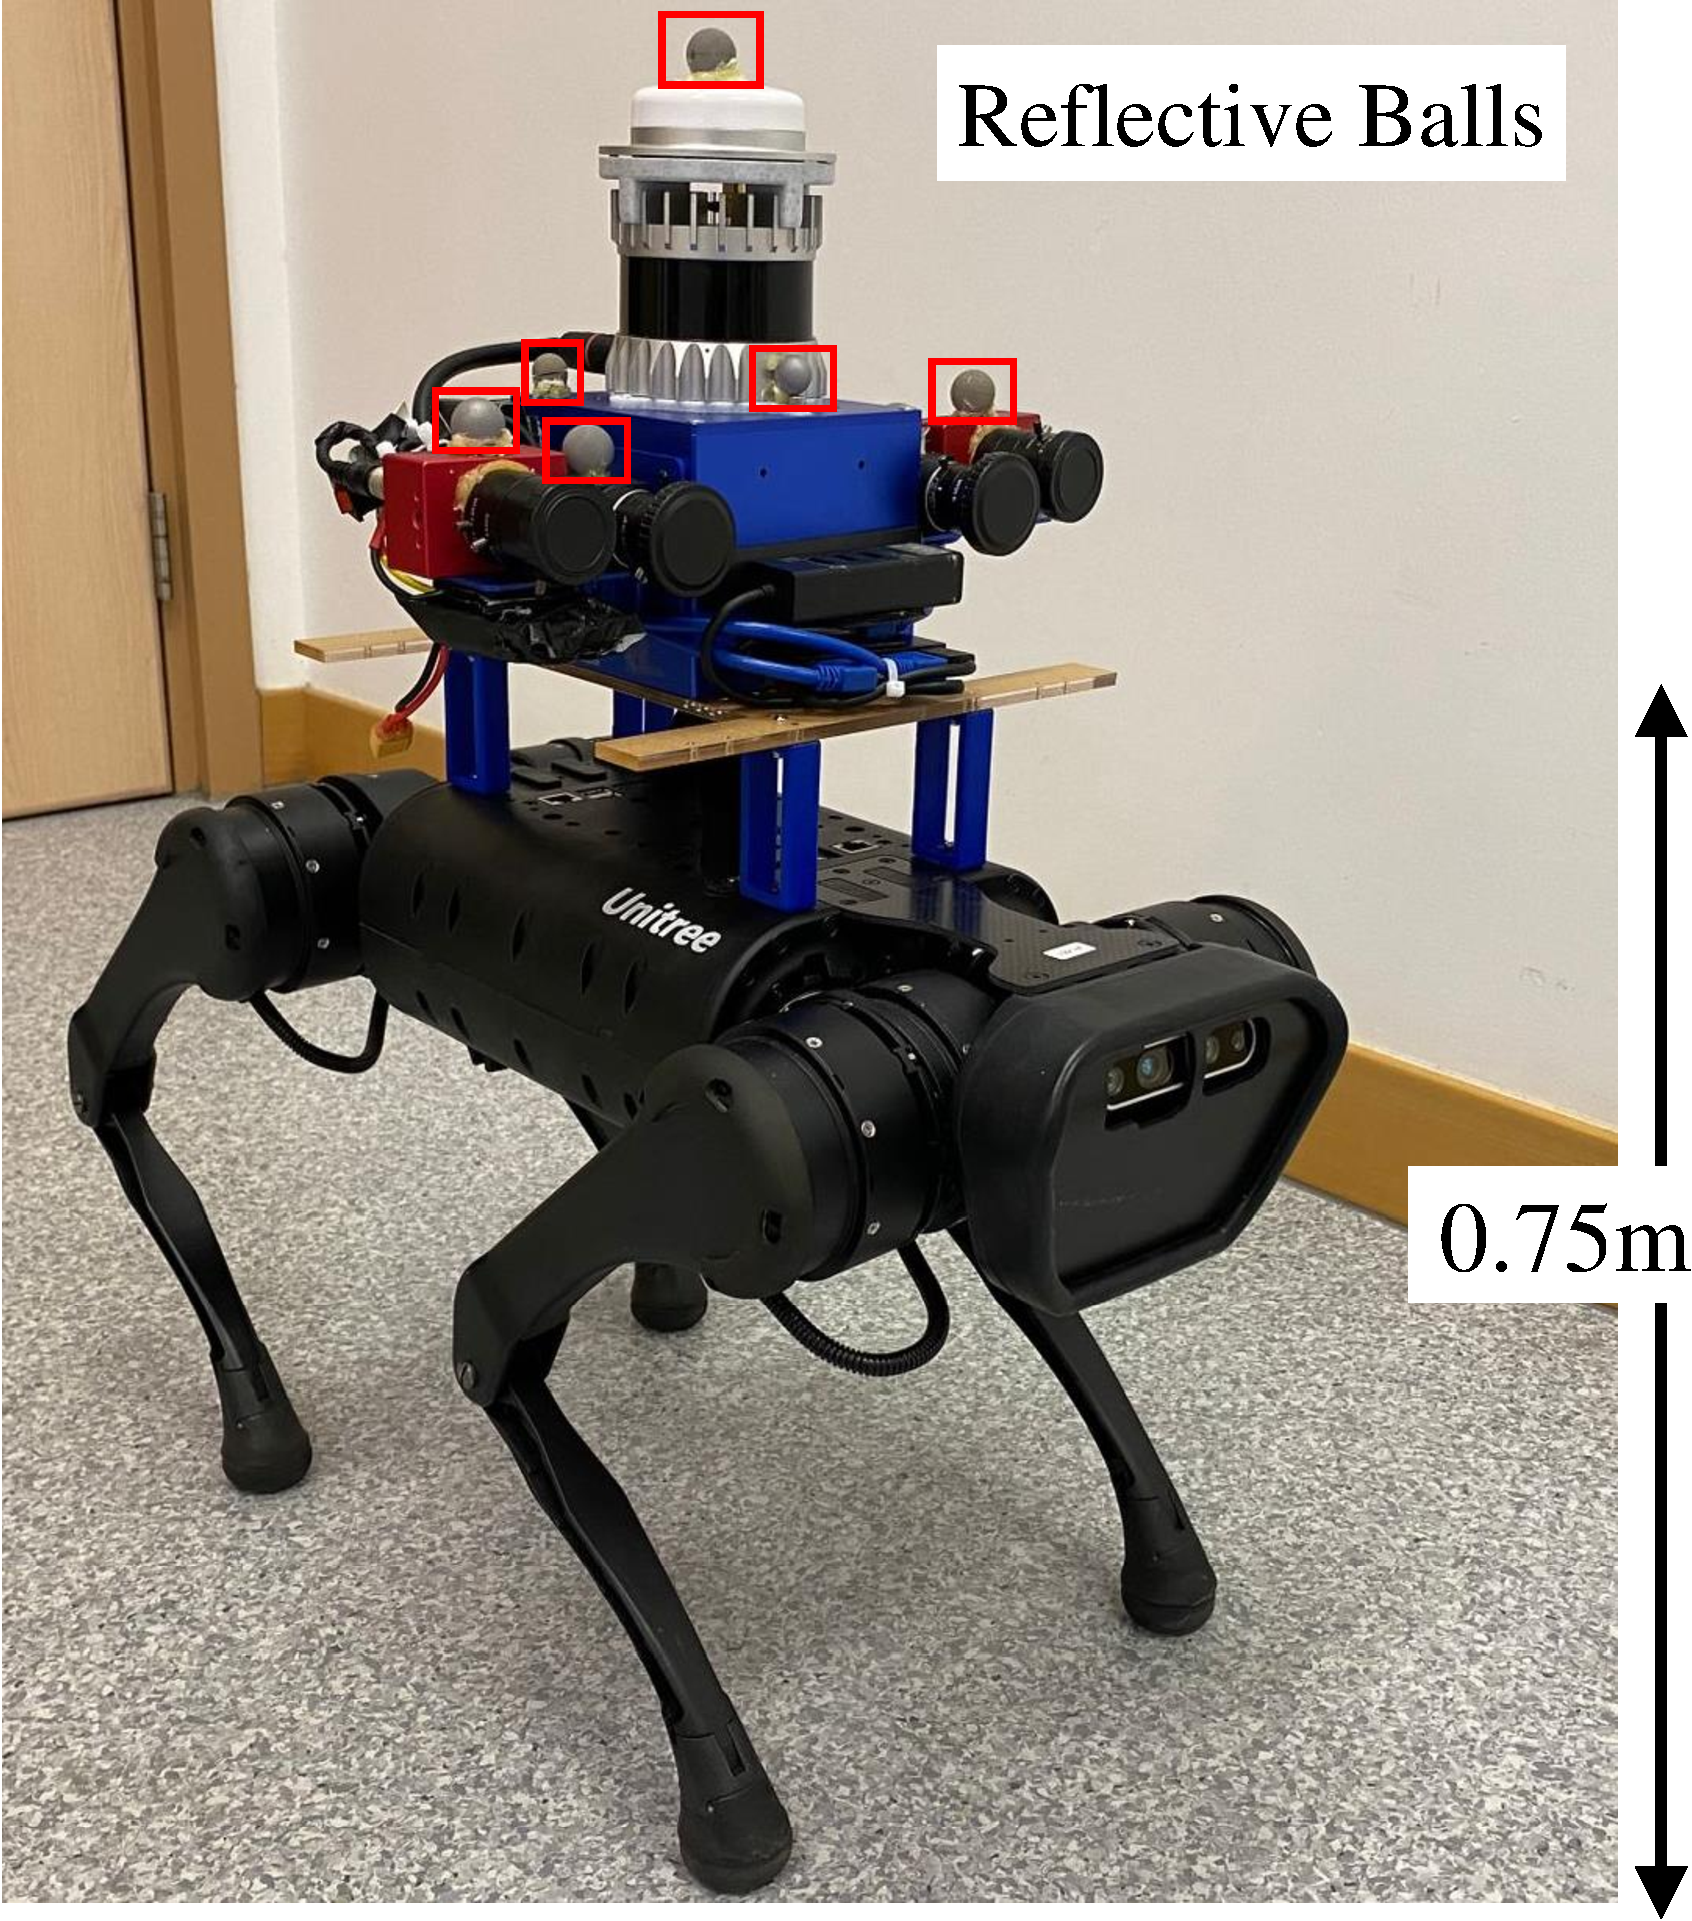
\includegraphics[width=.1776\linewidth]{figure/pqe/methodology/robotdog-crop.pdf}}
% \hspace{0.2cm}
% \end{subfigure}
% \begin{subfigure}
%     {\label{fig:sensor_apollo}\centering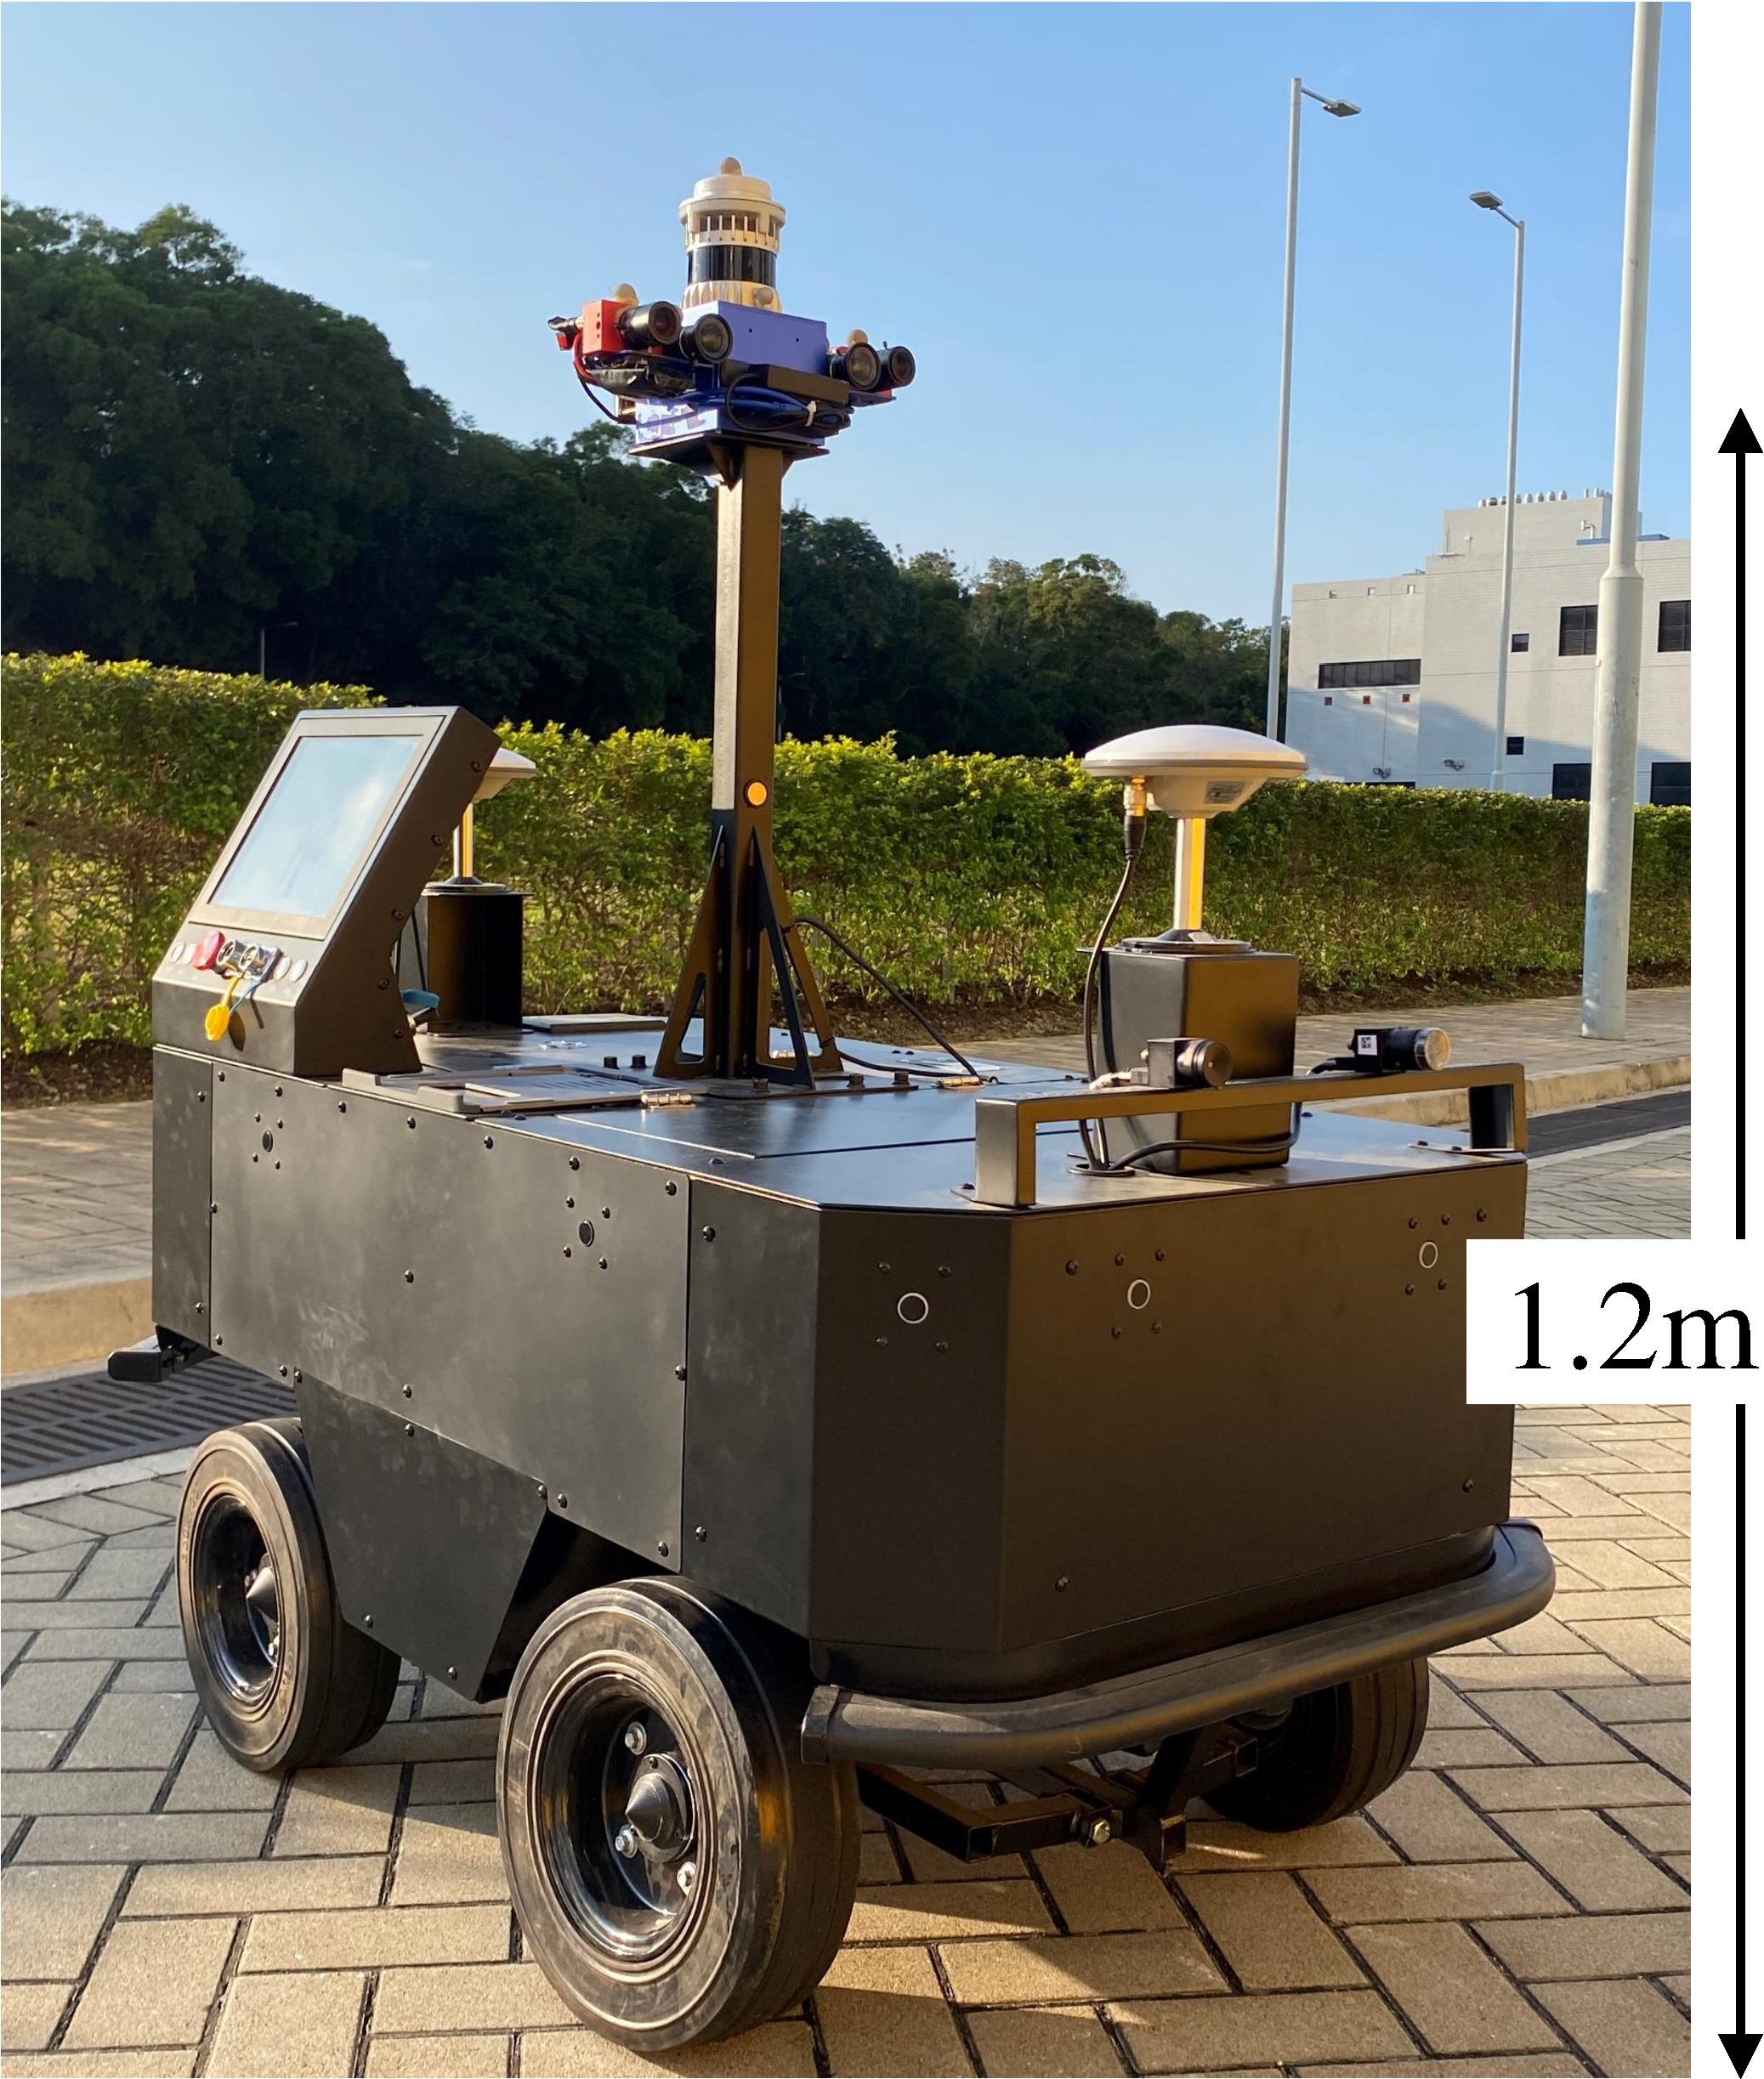
\includegraphics[width=.1701\linewidth]{figure/pqe/methodology/apollo-crop.pdf}} 
% \end{subfigure}
% \caption{The multi-sensor device and data collection platform: 
% (a) CAD model of the sensor rig, where axis directions are colored: red: $X$, green: $Y$, blue: $Z$. The sensor rig is rigidly mounted on (b) a gimbal stabilizer, (c) a quadruped robot, and (d) an apollo autonomous vehicle.}
% \label{fig:sensor_picture}
% \vspace{-0.3cm}
% \end{figure}  






% BIBLIOGRAPHY
\bibliographystyle{plain}
\bibliography{ref}

\end{document}
